%
% A header that lets you compile a chapter by itself, or inside a larger document.
% Adapted from http://stackoverflow.com/questions/3655454/conditional-import-in-latex
%
%
%Use \inbpdocument and \outbpdocument in your individual files, in place of \begin{document} and \end{document}. In your main file, put in a \def \ismaindoc {} before including or importing anything.
%
% David Duvenaud
% June 2011
% 
% ======================================
%
%


\ifx\ismaindoc\undefined
	\newcommand{\inbpdocument}{
		\def \ismaindoc {}
		% Use this header if we are compiling by ourselves.
		\documentclass[a4paper,11pt,authoryear,index]{common/PhDThesisPSnPDF}
		
%\usepackage{draftwatermark}
%\SetWatermarkLightness{0.95}

% ******************************************************************************
% ****************************** Custom Margin *********************************

% Add `custommargin' in the document class options to use this section
% Set {innerside margin / outerside margin / topmargin / bottom margin}  and
% other page dimensions

\ifsetMargin
\else
    \RequirePackage[left=37mm,right=30mm,top=35mm,bottom=30mm]{geometry}
    \setFancyHdr % To apply fancy header after geometry package is loaded
\fi


%\chead{Unfinished draft}
%\cfoot{\texttt{Unfinished draft - compiled on \today{} at \currenttime}}

% *****************************************************************************
% ******************* Fonts (like different typewriter fonts etc.)*************

% Add `customfont' in the document class option to use this section

\ifsetFont
\else
    % Set your custom font here and use `customfont' in options. Leave empty to
    % load computer modern font (default LaTeX font).  

    \RequirePackage{libertine} 
\fi

% *****************************************************************************
% *************************** Bibliography  and References ********************

%\usepackage{cleveref} %Referencing without need to explicitly state fig /table

% Add `custombib' in the document class option to use this section
\ifsetBib % True, Bibliography option is chosen in class options
\else % If custom bibliography style chosen then load bibstyle here

   \RequirePackage[square, sort, numbers, authoryear]{natbib} % CustomBib

% If you would like to use biblatex for your reference management, as opposed to the default `natbibpackage` pass the option `custombib` in the document class. Comment out the previous line to make sure you don't load the natbib package. Uncomment the following lines and specify the location of references.bib file

% \RequirePackage[backend=biber, style=numeric-comp, citestyle=numeric, sorting=nty, natbib=true]{biblatex}
% \bibliography{References/references} %Location of references.bib only for biblatex

\fi


% changes the default name `Bibliography` -> `References'
\renewcommand{\bibname}{References}


% *****************************************************************************
% *************** Changing the Visual Style of Chapter Headings ***************
% Uncomment the section below. Requires titlesec package.

%\RequirePackage{titlesec}
%\newcommand{\PreContentTitleFormat}{\titleformat{\chapter}[display]{\scshape\Large}
%{\Large\filleft{\chaptertitlename} \Huge\thechapter}
%{1ex}{}
%[\vspace{1ex}\titlerule]}
%\newcommand{\ContentTitleFormat}{\titleformat{\chapter}[display]{\scshape\huge}
%{\Large\filleft{\chaptertitlename} \Huge\thechapter}{1ex}
%{\titlerule\vspace{1ex}\filright}
%[\vspace{1ex}\titlerule]}
%\newcommand{\PostContentTitleFormat}{\PreContentTitleFormat}
%\PreContentTitleFormat


% *****************************************************************************
% **************************** Custom Packages ********************************
% *****************************************************************************


% ************************* Algorithms and Pseudocode **************************

%\usepackage{algpseudocode} 


% ********************Captions and Hyperreferencing / URL **********************

% Captions: This makes captions of figures use a boldfaced small font. 
%\RequirePackage[small,bf]{caption}

\RequirePackage[labelsep=space,tableposition=top]{caption} 
%\renewcommand{\figurename}{Figure} %to support older versions of captions.sty
\captionsetup{belowskip=12pt,aboveskip=4pt}

% ************************ Formatting / Footnote *******************************

%\usepackage[perpage]{footmisc} %Range of footnote options 


% ****************************** Line Numbers **********************************

%\RequirePackage{lineno}
%\linenumbers

% ************************** Graphics and figures *****************************

%\usepackage{rotating}
%\usepackage{wrapfig}
%\usepackage{float}
\usepackage{subfig} %note: subfig must be included after the `caption` package. 


% ********************************* Table **************************************

%\usepackage{longtable}
%\usepackage{multicol}
%\usepackage{multirow}
%\usepackage{tabularx}


% ***************************** Math and SI Units ******************************

\usepackage{amsfonts}
\usepackage{amsmath}
\usepackage{amssymb}
%\usepackage{siunitx} % use this package module for SI units


% ******************************************************************************
% ************************* User Defined Commands ******************************
% ******************************************************************************

% *********** To change the name of Table of Contents / LOF and LOT ************

%\renewcommand{\contentsname}{My Table of Contents}
%\renewcommand{\listfigurename}{List of figures}
%\renewcommand{\listtablename}{List of tables}


% ********************** TOC depth and numbering depth *************************

\setcounter{secnumdepth}{2}
\setcounter{tocdepth}{2}

% ******************************* Nomenclature *********************************

% To change the name of the Nomenclature section, uncomment the following line

%\renewcommand{\nomname}{Symbols}


% ********************************* Appendix ***********************************

% The default value of both \appendixtocname and \appendixpagename is `Appendices'. These names can all be changed via: 

%\renewcommand{\appendixtocname}{List of appendices}
%\renewcommand{\appendixname}{Appndx}

		% All my custom preamble stuff.  Shouldn't overlap with anything in official-preamble


% Paths to figure and table directories.
\newcommand{\symmetryfigsdir}{figures/symmetries}
\newcommand{\topologyfiguresdir}{figures/topology}
\newcommand{\infinitefiguresdir}{figures/infinite}
\newcommand{\grammarfiguresdir}{figures/grammar}
\newcommand{\introfigsdir}{figures/intro}
\newcommand{\gplvmfiguresdir}{figures/gplvm}
\newcommand{\warpedfiguresdir}{figures/warped-mixtures}
\newcommand{\deeplimitsfiguresdir}{figures/deep-limits}
\newcommand{\quadraturefigsdir}{figures/quadrature}
\newcommand{\additivefigsdir}{figures/additive}
\newcommand{\decompfigsdir}{figures/decomp}
\newcommand{\examplefigsdir}{figures/worked-example}


\usepackage{bm}  % for warped mixtures - is this necessary?
\usepackage{booktabs}
\usepackage{tabularx}
\usepackage{multirow}
\usepackage{datetime}
\renewcommand{\tabularxcolumn}[1]{>{\arraybackslash}m{#1}}
\usepackage{relsize}
\usepackage{graphicx}
\usepackage{amsmath,amssymb,textcomp}
\usepackage{nicefrac}
\usepackage{amsthm}
\usepackage{tikz}
\usetikzlibrary{arrows}
\usetikzlibrary{calc}
\usepackage{nth}
\usepackage{rotating}
\usepackage{array}
\usepackage{fp}
\usepackage[hyperpageref]{backref}
\def\foo{\hspace{\fill}\mbox{}\linebreak[0]\hspace*{\fill}}
\renewcommand*{\backref}[1]{}
\renewcommand*{\backrefalt}[4]{%
\ifcase #1 %
%
\or
\foo(page #2)%
\else
\foo(pages #2)%
\fi
}

\usepackage{cleveref}
\crefname{equation}{equation}{equations}


%% For submission, make all render blank.
%%%%%%%%%%%%%%%%%%%%%%%%%%%%%%%%%%%%%%%%%%%%%%%%%%%%%%%%%%
%%%% EDITING HELPER FUNCTIONS  %%%%%%%%%%%%%%%%%%%%%%%%%%%
%%%%%%%%%%%%%%%%%%%%%%%%%%%%%%%%%%%%%%%%%%%%%%%%%%%%%%%%%%

%% NA: needs attention (rough writing whose correctness needs to be verified)
%% TBD: instructions for how to fix a gap ("Describe the propagation by ...")
%% PROBLEM: bug or missing crucial bit 

%% use \fXXX versions of these macros to put additional explanation into a footnote.  
%% The idea is that we don't want to interrupt the flow of the paper or make it 
%% impossible to read because there are a bunch of comments.

%% NA's (and TBDs, those less crucially) should be written so 
%% that they flow with the text.

\definecolor{WowColor}{rgb}{.75,0,.75}
\definecolor{SubtleColor}{rgb}{0,0,.50}

% inline
\newcommand{\NA}[1]{\textcolor{SubtleColor}{ {\tiny \bf ($\star$)} #1}}
\newcommand{\LATER}[1]{\textcolor{SubtleColor}{ {\tiny \bf ($\dagger$)} #1}}
\newcommand{\TBD}[1]{\textcolor{SubtleColor}{ {\tiny \bf (!)} #1}}
\newcommand{\PROBLEM}[1]{\textcolor{WowColor}{ {\bf (!!)} {\bf #1}}}

% as margin notes

\newcounter{margincounter}
\newcommand{\displaycounter}{{\arabic{margincounter}}}
\newcommand{\incdisplaycounter}{{\stepcounter{margincounter}\arabic{margincounter}}}

\newcommand{\fTBD}[1]{\textcolor{SubtleColor}{$\,^{(\incdisplaycounter)}$}\marginpar{\tiny\textcolor{SubtleColor}{ {\tiny $(\displaycounter)$} #1}}}

\newcommand{\fPROBLEM}[1]{\textcolor{WowColor}{$\,^{((\incdisplaycounter))}$}\marginpar{\tiny\textcolor{WowColor}{ {\bf $\mathbf{((\displaycounter))}$} {\bf #1}}}}

\newcommand{\fLATER}[1]{\textcolor{SubtleColor}{$\,^{(\incdisplaycounter\dagger)}$}\marginpar{\tiny\textcolor{SubtleColor}{ {\tiny $(\displaycounter\dagger)$} #1}}}

%\renewcommand{\LATER}[1]{}
%\renewcommand{\fLATER}[1]{}
%\renewcommand{\TBD}[1]{}
%\renewcommand{\fTBD}[1]{}
%\renewcommand{\PROBLEM}[1]{}
%\renewcommand{\fPROBLEM}[1]{}
%\renewcommand{\NA}[1]{}


% HUMBLE WORDS: shown slightly smaller when in normal text
% Thanks to Christian Steinruecken!

% HUMBLE WORDS: shown slightly smaller when in normal text
%
\makeatletter%
%\def\@humbleformat#1{{\fontsize{}{1em}\selectfont #1}}
%\def\@humbleformat#1{\textsmaller{#1}}%
\newlength{\nonHumbleHeight}
\def\@humbleformat#1{{\settoheight{\nonHumbleHeight}{#1}\resizebox{!}{0.94\nonHumbleHeight}{#1}}}%
\def\@idxhumbleformat#1{{\relscale{0.95}{#1}}}%
%\def\@humbleformat#1{{#1}}%
\def\declareHumble#1#2{%
  \expandafter\def\csname #1\endcsname{\@humbleformat{#2}}%
  \expandafter\def\csname s#1\endcsname{{#2}}%
  \expandafter\def\csname idx#1\endcsname{{\@idxhumbleformat{#2}}}%
}%
\def\humble#1{\@humbleformat{#1}}%
\def\idxhumble#1{\@idxhumbleformat{#1}}%
\makeatother%

% Convenient indexing for humble abbreviations
\def\humbleindex#1#2{\index{#1@\idxhumble{#1}}}



% TODO: Clean up duplicates
\declareHumble{ANOVA}{ANOVA}
\declareHumble{ARD}{ARD}
\declareHumble{BIC}{BIC}
\declareHumble{BMC}{BMC}
\declareHumble{bq}{BQ}
\declareHumble{CRP}{CRP}
\declareHumble{dirpro}{DP}
\declareHumble{HDMR}{HDMR}
\declareHumble{GAM}{GAM}
\declareHumble{GEM}{GEM}
\declareHumble{GMM}{GMM}
\declareHumble{gplvm}{GP-LVM}
\declareHumble{gpml}{GPML}
\declareHumble{GPML}{GPML}
\declareHumble{gprn}{GPRN}
\declareHumble{gpt}{GP}
\declareHumble{gp}{GP}
\declareHumble{HKL}{HKL}
\declareHumble{HMC}{HMC}
\declareHumble{ibp}{IBP}
\declareHumble{iGMM}{iGMM}
\declareHumble{iwmm}{iWMM}
\declareHumble{kCP}{CP}
\declareHumble{kCW}{CW}
\declareHumble{kC}{C}
\declareHumble{KDE}{KDE}
\declareHumble{kLin}{Lin}
\declareHumble{KPCA}{KPCA}
\declareHumble{kPer}{Per}
\declareHumble{kRQ}{RQ}
\declareHumble{kSE}{SE}
\declareHumble{kWN}{WN}
\declareHumble{Lin}{Lin}
\declareHumble{LBFGS}{L-BFGS}
\declareHumble{mcmc}{MCMC}
\declareHumble{MKL}{MKL}
\declareHumble{MLP}{MLP}
\declareHumble{MSE}{MSE}
\declareHumble{Per}{Per}
\declareHumble{RMSE}{RMSE}
\declareHumble{RQ}{RQ}
\declareHumble{SBQ}{SBQ}
\declareHumble{seard}{SE-ARD}
\declareHumble{sefull}{SE-\textnormal{full}}
\declareHumble{SEGP}{SE-GP}
\declareHumble{SE}{SE}
\declareHumble{SNR}{SNR}
\declareHumble{SSANOVA}{SS-ANOVA}
\declareHumble{SVM}{SVM}

\newcommand{\kSig}{\boldsymbol\sigma}

\def\subexpr{{\cal S}}
\def\baseker{{\cal B}}
\def\numWinners{k}

\def\ie{i.e.\ }
\def\eg{e.g.\ }
\def\etc{etc.\ }
\let\oldemptyset\emptyset
\let\emptyset 0




% Unify notation between neural-net land and GP-land.
\newcommand{\hphi}{h}
\newcommand{\hPhi}{\vh}
\newcommand{\walpha}{w}
\newcommand{\wboldalpha}{\bw}
\newcommand{\wcapalpha}{\vW}
\newcommand{\lengthscale}{w}

\newcommand{\layerindex}{\ell}



\newcommand{\gpdrawbox}[1]{
\setlength\fboxsep{0pt}
\hspace{-0.15in} 
\fbox{
\includegraphics[width=0.464\columnwidth]{\deeplimitsfiguresdir/deep_draws/deep_gp_sample_layer_#1}
}}



\newcommand{\procedurename}{ABCD}
\newcommand{\genText}[1]{{\sf #1}}



\newcommand{\asdf}{$^{\textnormal{th}}$}

\newcommand{\binarysum}{\sum_{\bf{x} \in \{0,1\}^D}}
\newcommand{\expect}{\mathbb{E}}
\newcommand{\expectargs}[2]{\mathbb{E}_{#1} \left[ {#2} \right]}
\newcommand{\var}{\mathbb{V}}
\newcommand{\varianceargs}[2]{\mathbb{V}_{#1} \left[ {#2} \right]}
\newcommand{\cov}{\operatorname{cov}}
\newcommand{\Cov}{\operatorname{Cov}}
\newcommand{\covargs}[2]{\cov \left[ {#1}, {#2} \right]}
\newcommand{\variance}{\mathbb{V}}
\newcommand{\vecop}[1]{\operatorname{vec} \left( {#1} \right)}

\newcommand{\covarianceargs}[2]{\Cov_{#1} \left[ {#2} \right]}
\newcommand{\colvec}[2]{\left[ \begin{array}{c} {#1} \\ {#2} \end{array} \right]}
\newcommand{\tbtmat}[4]{\left[ \begin{array}{cc} {#1} & {#2} \\ {#3} & {#4} \end{array} \right]}

%\newcommand{\covskinny}[2]{\var\!\left(#1\middle\vert#2\right)} 

\newcommand{\acro}[1]{{\humble{#1}}}
%\newcommand{\vect}[1]{\boldsymbol{#1}}
\newcommand{\vect}[1]{{\bf{#1}}}
\newcommand{\mat}[1]{\mathbf{#1}}
\newcommand{\pderiv}[2]{\frac{\partial #1}{\partial #2}}
\newcommand{\npderiv}[2]{\nicefrac{\partial #1}{\partial #2}}

\newcommand{\pha}{^{\phantom{:}}}

\newcommand{\argmin}{\operatornamewithlimits{argmin}}
\newcommand{\argmax}{\operatornamewithlimits{argmax}}

% The following designed for probabilities with long arguments

\newcommand{\Prob}[2]{P\!\left(\,#1\;\middle\vert\;#2\,\right)}
\newcommand{\ProbF}[3]{P\!\left(\,#1\!=\!#2\;\middle\vert\;#3\,\right)}
\newcommand{\p}[2]{p\!\left(#1\middle\vert#2\right)}
\newcommand{\po}[1]{p\!\left(#1\right)}
\newcommand{\pF}[3]{p\!\left(\,#1\!=\!#2\;\middle\vert\;#3\,\right)} 
\newcommand{\mean}[2]{{m}\!\left(#1\middle\vert#2\right)}



\newcommand{\valpha}{\boldsymbol{\alpha}}
\newcommand{\va}{\vect{a}}
\newcommand{\vA}{\vect{A}}
\newcommand{\vB}{\mat{B}}
\newcommand{\vb}{\vect{b}}
\newcommand{\vC}{\mat{C}}
\newcommand{\vc}{\vect{c}}
\newcommand{\vecf}{\boldsymbol{f}}
\newcommand{\vell}{\vect{\ell}}
\newcommand{\vepsilon}{\boldsymbol{\epsilon}}
\newcommand{\veps}{\boldsymbol{\epsilon}}
\newcommand{\ve}{\boldsymbol{\epsilon}}
\newcommand{\vf}{\vecf}
\newcommand{\vg}{\vect{g}}
\newcommand{\vh}{\vect{h}}
\newcommand{\vI}{\mat{I}}
\newcommand{\vK}{\mat{K}}
\newcommand{\vk}{\vect{k}}
\newcommand{\vL}{\mat{L}}
\newcommand{\vl}{\vect{l}}
\newcommand{\vmu}{\boldsymbol{\mu}}
\newcommand{\vone}{\vect{1}}
\newcommand{\vphi}{\boldsymbol{\phi}}
\newcommand{\vpi}{\boldsymbol{\pi}}
\newcommand{\vq}{\vect{q}}
\newcommand{\vR}{\mat{R}}
\newcommand{\vr}{\vect{r}}
\newcommand{\vsigma}{\boldsymbol{\sigma}}
\newcommand{\vSigma}{\mat{\Sigma}}
\newcommand{\vS}{\mat{S}}
\newcommand{\vs}{\vect{s}}
\newcommand{\vtheta}{\boldsymbol{\theta}}
\newcommand{\vu}{\vect{u}}
\newcommand{\vV}{\mat{V}}
\newcommand{\vW}{\mat{W}}
\newcommand{\vw}{\vect{w}}
\newcommand{\vX}{\mat{X}}
\newcommand{\vx}{\vect{x}}
\newcommand{\vY}{\mat{Y}}
\newcommand{\vy}{\vect{y}}
\newcommand{\vzero}{\vect{0}}
\newcommand{\vZ}{\mat{Z}}
\newcommand{\vz}{\vect{z}}


\newcommand{\netweights}{\alpha}
\newcommand{\vnetweights}{\valpha}

\newcommand{\He}{\mathcal{H}}
\newcommand{\normx}[2]{\left\|#1\right\|_{#2}}
\newcommand{\Hnorm}[1]{\normx{#1}{\He}}
\newcommand{\mmd}{{\rm MMD}}


\newcommand{\mf}{\bar{\vf}}

%\newcommand{\mf}{\mu} %{\bar{\ell}}
\newcommand{\lf}{f} % Likelihood function
\newcommand{\st}{_\star}

% from simpler log-bq writeup
\newcommand{\lftwo}{{\log \ell}}
\newcommand{\mftwo}{{\bar \ell}}
\newcommand{\loggp}{{\log\acro{GP}}}%| \bX, \vy )}}
\newcommand{\loggpdist}{{\acro{GP}(\lftwo)}}%| \vX, \vy )}}


\newcommand{\inv}{^{{\mathsmaller{-1}}}}
\newcommand{\tohalf}{^{{\mathsmaller{\nicefrac{1}{2}}}}}

\newcommand{\Normal}{\mathcal{N}}
\newcommand{\N}[3]{\mathcal{N}\!\left(#1 \middle| #2,#3\right)}
\newcommand{\Nt}[2]{\mathcal{N}\!\left(#1,#2\right)}
\newcommand{\NT}[2]{\mathcal{N}\!\left(#1,#2\right)}
\newcommand{\GPdist}[3]{\mathcal{GP}\!\left(#1 \, \middle| \, #2, #3 \right)}
\newcommand{\bN}[3]{\mathcal{N}\big(#1 \middle| #2,#3\big)}
\newcommand{\boldN}[3]{\text{\textbf{\mathcal{N}}}\big(#1;#2,#3\big)}
\newcommand{\ones}[1]{\mat{1}_{#1}}
\newcommand{\eye}[1]{\mat{E}_{#1}}
\newcommand{\tra}{^{\mathsf{T}}}
%\newcommand{\tra}{^{\top}}
%\mathsf{T}
\newcommand{\trace}{\operatorname{tr}}
\newcommand{\shift}{\operatorname{shift}}
\renewcommand{\mod}{\operatorname{mod}}
\newcommand{\deq}{:=}
\newcommand{\oneofk}{\operatorname{one-of-k}}
%\newcommand{\degree}{^\circ}

\newcommand{\GPt}[2]{\mathcal{GP}\!\left(#1,#2\right)}
%\newcommand{\GPt}[2]{\gp\!\left(#1,#2\right)}

\DeclareMathOperator{\tr}{tr}
\DeclareMathOperator{\chol}{chol}
\DeclareMathOperator{\diag}{diag}

\newenvironment{narrow}[2]{%
  \begin{list}{}{%
  \setlength{\topsep}{0pt}%
  \setlength{\leftmargin}{#1}%
  \setlength{\rightmargin}{#2}%
  \setlength{\listparindent}{\parindent}%
  \setlength{\itemindent}{\parindent}%
  \setlength{\parsep}{\parskip}}%
\item[]}{\end{list}}



\newcommand{\dist}{\ \sim\ }
\def\given{\,|\,}

% Table stuff
\newcolumntype{C}[1]{>{\centering\let\newline\\\arraybackslash\hspace{0pt}}m{#1}}
\newcolumntype{L}[1]{>{\raggedright\let\newline\\\arraybackslash\hspace{0pt}}m{#1}}
\newcolumntype{R}[1]{>{\raggedleft\let\newline\\\arraybackslash\hspace{0pt}}m{#1}}


\def\ie{i.e.\ }
\def\eg{e.g.\ }
\def\iid{i.i.d.\ }
%\def\simiid{\sim_{\mbox{\tiny iid}}}
\def\simiid{\overset{\mbox{\tiny iid}}{\sim}}
\def\simind{\overset{\mbox{\tiny \textnormal{ind}}}{\sim}}
\def\eqdist{\stackrel{\mbox{\tiny d}}{=}}
%\newcommand{\distas}[1]{\mathbin{\overset{#1}{\kern \z@ \sim}}}
%TODO: fix this - it worked outside the thesis!
\newcommand{\distas}[1]{\mathbin{\overset{#1}{\sim}}}

\def\Reals{\mathbb{R}}

\def\Uniform{\mbox{\rm Uniform}}
\def\Bernoulli{\mbox{\rm Bernoulli}}
\def\GP{\mathcal{GP}}
\def\GPLVM{\mathcal{GP-LVM}}




% Kernel stuff

\def\iva{\vect{\inputVar}}
\def\ivaone{\inputVar}
\def\inputVar{x}
\def\InputVar{X}
\def\InputSpace{\mathcal{X}}
\def\outputVar{y}
\def\OutputSpace{\mathcal{Y}}
\def\function{f}
\def\kernel{k}
\def\KernelMatrix{K}
\def\SumKernel{\sum}
\def\ProductKernel{\prod}
\def\expression{e}
\def\feat{\vh}

\newcommand{\kerntimes}{ \! \times \!}
\newcommand{\kernplus}{ \, + \,}


% Proof stuff
\theoremstyle{plain}
\newtheorem{theorem}{Theorem}[section]
\newtheorem{lemma}[theorem]{Lemma}
\newtheorem{prop}[theorem]{Proposition}
\newtheorem{proposition}{Proposition}
\newtheorem*{cor}{Corollary}

% For infinite bq
\newcommand{\iv}{\theta}
\newcommand{\viv}{\vtheta}

% For intro chapter
\newcommand{\funcval}{\vf(\vX)}
\newcommand{\testpoint}{{\vx^\star}}

\newcommand{\underwrite}[2]{{\underbrace{#1}_{\textnormal{#2}}}}



% For kernel figures
\newcommand{\fhbig}{2cm}%
\newcommand{\fwbig}{3cm}%
\newcommand{\kernpic}[1]{\includegraphics[height=\fhbig,width=\fwbig]{\grammarfiguresdir/structure_examples/#1}}%
\newcommand{\kernpicr}[1]{\rotatebox{90}{\includegraphics[height=\fwbig,width=\fhbig]{\grammarfiguresdir/structure_examples/#1}}}%
\newcommand{\addkernpic}[1]{{\includegraphics[height=\fhbig,width=\fwbig]{\grammarfiguresdir/additive_multi_d/#1}}}%
\newcommand{\largeplus}{\tabbox{{\Large+}}}%
\newcommand{\largeeq}{\tabbox{{\Large=}}}%
\newcommand{\largetimes}{\tabbox{{\Large$\times$}}}%
\newcommand{\fixedx}{$x$ (with $x' = 1$)}%


		% ************************ Thesis Information & Meta-data **********************

%% The title of the thesis
%\title{Structured Gaussian Process Models} 
%\title{Automatic Model Construction \\ through \\ Structured Gaussian Processes}
%\title{Automatic Model-Building \\ through \\ Structured Gaussian Processes}
%\title{Automatic Modeling \\ with \\ Structured Gaussian Processes}    
\title{Automatic Model Construction \\ with Gaussian Processes}
%\title{Automatic Model Construction}
%\title{Automating Statistical Model Construction}


%\texorpdfstring is used for PDF metadata. Usage:
%\texorpdfstring{LaTeX_Version}{PDF Version (non-latex)} eg.,
%\texorpdfstring{$sigma$}{sigma}

%% The full name of the author
\author{David Kristjanson Duvenaud}

%% Department (eg. Department of Engineering, Maths, Physics)
%\dept{Department of Engineering}

%% University and Crest
\university{University of Cambridge}
\crest{
\includegraphics[width=0.25\textwidth]{University_Crest}}

%% You can redefine the submission text:
% Default as per the University guidelines: This dissertation is submitted for
% the degree of Doctor of Philosophy
%\renewcommand{\submissiontext}{change the default text here if needed}

%% Full title of the Degree 
\degree{Doctor of Philosophy}
 
%% College affiliation (optional)
\college{Pembroke College}

%% Submission date
\degreedate{June 2014} 

%% Meta information
\subject{LaTeX} \keywords{{LaTeX} {PhD Thesis} {Engineering} {University of Cambridge}}



		\begin{document}
	}	
	\newcommand{\outbpdocument}[1]{

		% Fake chapters so references aren't broken
\label{ch:intro}                
\label{ch:kernels}
\label{ch:grammar}
\label{ch:description}
\label{ch:additive}
\label{ch:deeplimits}
\label{ch:discussion}
		%\bibliographystyle{common/CUEDthesis}
		\bibliographystyle{plainnat}
		\bibliography{references.bib}
		\end{document}
	}	
\else
	%If we're inside another document, no need to re-start the document.
	\ifx\inbpdocument\undefined
		\newcommand{\inbpdocument}{}
		\newcommand{\outbpdocument}[1]{}
	\fi
\fi

\inbpdocument


\chapter{Automatically Building Structured Covariance Functions}
\label{ch:grammar}

\begin{quotation}
``It would be very nice to have a formal apparatus that gives us some `optimal' way of recognizing unusual phenomena and inventing new classes of hypotheses that are most likely to contain the true one; but this remains an art for the creative human mind.''
% In trying to practice this art, the Bayesian has the advantage because his formal apparatus already developed gives him a clearer picture of what to expect, and therefore a sharper perception for recognizing the unexpected.

\defcitealias{Jaynes85highlyinformative}{E. T.  Jaynes, 1985}
\hspace*{\fill}\citetalias{Jaynes85highlyinformative}
\end{quotation}


In \cref{ch:kernels}, we saw that the choice of kernel determines the type of structure that can be learnt by a \gp{} model.
We also saw that a wide variety of models could be constructed through simply adding and multiplying a few base kernels together.
%Applying \gp{} regression as a non-expert is a daunting task.
However, when facing a new problem, it is sometimes difficult to construct an appropriate kernel by hand.
%The first problem one encounters when attempting to apply \gp{}s to a particular task is that the choice of kernel is very important, but it's usually not clear which covariance function is appropriate.
Even for experts, choosing the kernel in nonparametric regression remains something of a black art.

%As we shall see in this thesis, in the small-to-medium data range, the choice of of kernel is extremely important.
%This is especially true when one wishes to do extrapolation.

%When I first used the GPML package, I was stymied by the lack of a default kernel.
%Faced with a bewildering array of possible kernels to try, I simply tried each one, and chose the one with the best predictive performance on a held-out test set.
%Why not simply automate this process as part of the software package?
%After starting my Ph.D., 

In this chapter, we'll automate this process.

%e define a space of kernel structures which are built compositionally by adding and multiplying a small number of base kernels.
We present a method for searching over this space of structures which mirrors the scientific discovery process.
The learned structures can often decompose functions into interpretable components and enable long-range extrapolation on time-series datasets.
Our structure search method outperforms many widely used kernels and kernel combination methods on a variety of prediction tasks.



This paper presents the beginnings of an automatic statistician, focusing on regression problems.
Our system explores an open-ended space of possible statistical models to discover a good explanation of the data, and then produces a detailed report with figures and natural-language text.

Our approach treats unknown functions nonparametrically using Gaussian processes, which has two important consequences.
First, Gaussian processes model functions in terms of high-level properties (e.g.\ smoothness, trends, periodicity,
changepoints).
Taken together with the compositional structure of our language of models, this allows us to automatically describe functions through a decomposition into additive parts.
Second, the use of flexible nonparametric models and a rich language for composing them in an open-ended manner also results in state-of-the-art extrapolation performance evaluated over 13 real time series data sets from various domains.


%\subsection{Attribution}
% Moved to first chapter.
%Joint work with James Robert Lloyd, Roger Grosse, Joshua B. Tenenbaum and Zoubin Ghahramani.


%\section{Introduction}

%Supervised learning problems, such as classification and regression, learn a function $\function$ from some input (predictor) variables, $\InputVar$, to some output (response) variables, $\outputVar$.
%Kernel-based nonparametric models, such as support vector machines and Gaussian processes (\gp{}s), have been one of the dominant paradigms for supervised machine learning over the last 20 years.
%These methods depend on defining a kernel function, $\kernel(\inputVar,\inputVar')$, which specifies how similar or correlated outputs $\outputVar$ and $\outputVar'$ are expected to be at two inputs $\inputVar$ and $\inputVar'$.
By defining the measure of similarity between inputs, the kernel determines the pattern of inductive generalization.
%The kernel function gives a measure of similarity between inputs and determines the pattern of inductive generalizations that are made. 

Most existing techniques pose kernel learning as a (possibly high-dimensional) parameter estimation problem.
%The ability to learn kernels automatically has helped greatly in making kernel methods accessible to non-experts.
Examples include learning hyperparameters \citep{rasmussen38gaussian}, linear combinations of fixed kernels \cite{Bach_HKL}, and mappings from the input space to an embedding space \cite{salakhutdinov2008using}.

However, to apply existing kernel learning algorithms, the user must specify the parametric form of the kernel, and this can require considerable expertise, as well as trial and error.

To make kernel learning more generally applicable, we reframe the kernel learning problem as one of structure discovery, and automate the choice of kernel form.
In particular, we formulate a space of kernel structures defined compositionally in terms of sums and products of a small number of base kernel structures.
This provides an expressive modeling language which concisely captures many widely used techniques for constructing kernels.
%We focus on Gaussian process regression, where the kernel specifies a covariance function, because the Bayesian framework is a convenient way to formalize structure discovery.
Borrowing discrete search techniques which have proved successful in equation discovery \cite{todorovski1997declarative} and unsupervised learning \cite{grosse2012exploiting}, we automatically search over this space of kernel structures using marginal likelihood as the search criterion.

This simple structure discovery algorithm is able to automatically recover known structures from synthetic data as well as plausible structures for a variety of real-world datasets. 
On a variety of time series datasets, the learned kernels yield decompositions of the unknown function into interpretable components that enable accurate extrapolation beyond the range of the observations.
Furthermore, the automatically discovered kernels outperform a variety of widely used kernel classes and kernel combination methods on supervised prediction tasks.

%\fTBD{I hate these paragraphs, but they seem to be required...} 
%Section \ref{sec:Structure} outlines some commonly used kernel families as well as ways in which they can be composed. 
%Our grammar over kernels and our proposed structure discovery algorithm are described in Section \ref{sec:Search}. 
%Section \ref{sec:related_work} situates our work in the context of other nonparametric regression, kernel learning, and structure discovery methods.
%We evaluate our methods on synthetic datasets, time series analysis, and high-dimensional prediction problems in Sections \ref{sec:synthetic} through \ref{sec:quantitative}, respectively.




%Kernel learning has been an important topic in machine learning since the kernel essentially determines the pattern of inductive
%generalisation \fTBD{which citations canonical?}\citep[e.g.][]{diosan2007evolving,salakhutdinov2008using,Bach_HKL}.
%In this paper, we pose the problem of kernel learning in a radically new way, as one of structure discovery from data.
%In previous work, kernel learning has been posed as a problem of (possibly very high-dimensional) parameter estimation.
%Here we reframe the problem of kernel learning as one of structure discovery from data.
%This provides a more expressive modeling language, allows us to exploit efficient discrete search methods that rapidly explore a large space of structures, and yields results that are both more interpretable and better in objective generalization performance.
%A key challenge for kernel based methods is learning an appropriate kernel from data, and a great many papers have been written on this important topic\TBD{ cite kernel learning for SVMs and GP literature}. \TBD{RBG: sounds like another approach to the same problem; want it to be an underexplored \emph{aspect} of the problem}
%In this paper, we pose the problem of kernel learning as a problem of structure discovery from data.

%We use this insight to define a simple grammar over composite kernels, and we develop an automated search algorithm over the (exponentially large) space of kernels that can be derived from this grammar.
%The search criterion is the marginal likelihood of the kernel, which is the driving term for Bayesian model comparison and selection in analogous structure discovery tasks such as graphical model learning \cite{heckerman1995learning}.

%\paragraph{Benefits of kernel structure}  In many regression problems, or time series analysis, or when modeling dynamical systems, we often think we are observing the superposition of multiple distinct causal processes.
%For example, an underlying linear function plus Gaussian noise in classical linear regression, or an underlying linear dynamics plus Gaussian observation noise in a Kalman filter.
%Our approach can be seen as a general way to learn functions like this, where the product of kernels can be used to capture richer causal proceses (e.g., nonlinear rather simply linear, amplifying perioidic (as in the second layer of the airline example) rather than simply periodic) and the sum of kernels corresponds to the superposition of these causal processes.


% Moved to discussion.
%Automating the process of statistical modeling would have a tremendous impact on fields that currently rely on expert statisticians, machine learning researchers, and data scientists.
%While fitting simple models (such as linear regression) is largely automated by standard software packages, there has been little work on the automatic construction of flexible but interpretable models. 

%What are the ingredients required for an artificial intelligence system to be able to perform statistical modeling automatically? 
%In this paper we conjecture that the following ingredients may be useful for building an AI system for statistics, and we develop a working system which incorporates them:
%\begin{itemize}
%\item {\bf An open-ended language of models} expressive enough to capture many of the modeling assumptions and model composition techniques  applied by human statisticians to capture real-world phenomena
%\item {\bf A search procedure} to efficiently explore the space of models spanned by the language
%\item {\bf A principled method for evaluating models} in terms of their complexity and their degree of fit to the data
%\item {\bf A procedure for automatically generating reports} which can explain and visualize different factors underlying the data, make the chosen modeling assumptions explicit, and quantify how each component improves the predictive power of the model 
%\end{itemize}


\section{Ingredients of an Automatic Statistician}
\label{sec:ingredients}
%\fTBD{JL: Has RG written anything on this?}
\citet{gelman2013philblogpost} asks ``How can an artificial intelligence do statistics? ... It needs not just an inference engine, but also a way to construct new models and a way to check models. Currently, those steps are performed by humans, but the AI would have to do it itself.''

%In this section, we discuss in more detail the elements required to build a system that can automatically construct and then describe complex nonparametric models.

In this section, we discuss in more detail the elements we believe are required to build an artificial intelligence that can do statistics.

\paragraph{1. An open-ended language of models}
Many statistical procedures consider all models in a class of fixed size - for example, graphical model construction algorithms\fTBD{Cite} search over connectivity graphs for a given set of nodes.
While these methods can be powerful, human statisticians are capable of deriving novel model classes when required by the modelling task.
%An open ended language can 
An automatic search through an open-ended class of models can achieve some of this flexibility, growing the complexity of the model to fit the task at hand, and possibly combining existing structures in novel ways.
%However, in order for a procedure to be as powerful as a human statistician, it must be able to add to a model in a wide variety of ways, building arbitrarily complex models if the data demands it.

\paragraph{2. Searching through model space}
An open-ended space of models cannot be searched exhaustively.
Just as human researchers iteratively refine their models, search procedures can propose new search directions based on the results of previous model fits.
Because any search in an open-ended space must start with relatively simple models before moving on to more complex ones, any model search in an open-ended space will likely resemble a model-building procedure.% based 

\paragraph{3. Model comparison and checking model fit}
An automatic statistician should be able to question the models it has constructed, and formal procedures from model checking provide a way for it to do this.
%A practically and philsophically interesting question is how to compare models, and how to check whether there is statistical structure not being captured by a given model. 
%\fTBD{Struggling with this section - do we need to defend marginal likelihood or discuss the options}
\citet{gelman2012philosophy} review the literature on model checking.
In this work, we use approximate marginal likelihood to compare models, penalizing complexity using the Bayesian Information Criterion as a heuristic.

\paragraph{4. Describing models}

%Capturing statistical structure helps to provide good predictions. 
Part of the value of statistical models comes from enabling humans to understand a dataset or a phenomenon.
Furthermore, a clear description of the statistical structure found in a dataset helps a user to notice when the dataset has errors, the wrong question was asked, the model-building procedure failed to capture known structure, a relevant piece of data or constraint is missing, or when a novel statistical structure has been found.

%It is not clear\fTBD{JL: Weak} what obstacles there are to building a system capable of explaining novel statistical structures.
We
%attempted to build such an automatic summarization procedure, and 
demonstrate that the properties of Gaussian processes allow for an automatic, modular description generation procedure, trhough both graphs illustrating interpretable decomposition of the posterior, and in terms of English-language descriptions of properties of the discovered models.
%This modularity means that a large class of statistical structures can explained, without resorting to writing a special case for every possible structure in our open-ended set of models.

Whether or not such modularity and interpretability is present in other open-ended model classes is an open question.



In this chapter, we introduce a system for modeling time-series data containing the above ingredients which we call the Automatic Bayesian Covariance Discovery (\procedurename{}) system.
The system defines an open-ended language of Gaussian process models via a compositional grammar.
The space is searched greedily, using marginal likelihood and the Bayesian Information Criterion (BIC) to evaluate models.
The compositional structure of the language allows us to develop a method for automatically translating components of the model into natural-language descriptions of patterns in the data.

We show examples of automatically generated reports which highlight interpretable features discovered in a variety of data sets (e.g.\ Figure~\ref{fig:periodic}).
%The supplementary material to this paper includes 13 complete reports automatically generated by \procedurename{}.

Good statistical modeling requires not only interpretability but predictive accuracy.
We compare \procedurename{} against existing model construction techniques in terms of predictive performance at extrapolation, and we find state-of-the-art performance on 13 time series.





\section{A Language of Regression Models}
\label{sec:improvements}



As shown in Chapter~\ref{ch:kernels}, we can construct a wide variety of kernel structures compositionally by adding and multiplying a small number of base kernels.
In particular, we consider the four base kernel families discussed in Section \ref{sec:Structure}: \kSE, \kPer, \kLin, and \kRQ.
Any algebraic expression combining these kernels using the operations $+$ and $\times$ defines a kernel family, whose parameters are the concatenation of the parameters for the base kernel families. 




%Details of the search algorithm are given in the supplementary material \TBD{For now}.

%\paragraph{A greedy search algorithm}
%Our search starts by first proposing all base kernels applied to all input dimensions.  We then choose the kernel with the highest approximate marginal likelihood, apply all expansions to this kernel, and repeat this process for a fixed number of steps.





%The general problem of regression consists of learning a function $f$ mapping from some input space $\mathcal{X}$ to some output space $\mathcal{Y}$.
We would like an expressive language which can represent both simple parametric forms of $f$ such as linear, polynomial, \etc and also complex nonparametric functions specified in terms of properties such as smoothness, periodicity, \etc~
Fortunately, Gaussian processes (\gp{}s) provide a very general and analytically tractable way of capturing both simple and complex functions. 

%Gaussian processes are distributions over functions such that any finite subset of function evaluations, $(f(x_1), f(x_2), \ldots f(x_N))$, have a joint Gaussian distribution \citep{rasmussen38gaussian}.
%A \gp{} is completely specified by its mean function, $\mu(x)=\mathbb{E}(f(x))$ and kernel (or covariance) function $\kernel(x,x') = \Cov(f(x),f(x'))$.
%It is common practice to assume zero mean, since marginalizing over an unknown mean function can be equivalently expressed as a zero-mean \gp{} with a new kernel.
%The structure of the kernel captures high-level properties of the unknown function, $f$, which in turn determines how the model generalizes or extrapolates to new data.

We can therefore define a language of regression models by specifying a language of kernels.

The elements of this language are a set of  base kernels capturing different function properties, and a set of
composition rules which combine kernels to yield other valid kernels.
Our base kernels are white noise ($\kWN$), constant ($\kC$), linear ($\kLin$), squared exponential ($\kSE$) and periodic ($\kPer$), which on their own encode for uncorrelated noise, constant functions, linear functions, smooth functions and periodic functions respectively.
%\footnote{Definitions of kernels are in the supplementary material.}.
The composition rules are addition and multiplication:
\begin{align}
k_1 + k_2 =      & \,\, k_1(x,x') + k_2(x,x') \\
k_1 \times k_2 = & \,\, k_1(x,x') \times k_2(x,x')
\end{align}

%Combining kernels using these operations can yield kernels encoding for richer structures such as approximate periodicity ($\kSE \times \kPer$) or smooth functions with linear trends ($\kSE + \kLin$).

%This kernel composition framework (with different base kernels) was described by \citet{DuvLloGroetal13}.
%We extend and adapt this framework in several ways.
We have found that incorporating changepoints into the language is essential for realistic models of time series (\eg figure~\ref{fig:periodic}).

% Moved to kernels chapter.
%Changepoints can be defined through addition and multiplication with sigmoidal functions:
%\begin{align}
%\kCP(\kernel_1, \kernel_2) = \kernel_1 \times \boldsymbol\sigma + \kernel_2 \times \boldsymbol{\bar\sigma}
%\label{eq:cp}
%\end{align}
%where $\boldsymbol\sigma = \sigma(x)\sigma(x')$ and $\boldsymbol{\bar\sigma} = (1-\sigma(x))(1-\sigma(x'))$.
%Changewindows $\kCW(\cdot,\cdot)$ can be defined similarly by replacing $\sigma(x)$ with a product of two sigmoids.

%We also expanded and reparametrised the set of base kernels so that they were more amenable to automatic description and to extend the number of common regression models included in the language.

Table~\ref{table:motifs} lists common regression models that can be expressed by our language.
\begin{table}[ht]
\centering
\begin{tabular}{l|l}
Regression model & Kernel \\
\midrule
Linear regression & $\kC + \kLin + \kWN$ \\
Kernel ridge regression & $\kSE + \kWN$ \\
Multiple kernel learning & $\sum \kSE$ + \kWN\\
Trend, cyclical, irregular & $\sum \kSE + \sum \kPer$ + \kWN\\
Fourier decomposition & $\kC + \sum \cos$ + \kWN\\
Sparse spectrum \gp{}s & $\sum \cos$ + \kWN\\
Spectral mixture & $\sum \SE \times \cos$ + \kWN\\
Changepoints & \eg $\kCP(\kSE, \kSE) + \kWN$ \\
Heteroscedasticity & \eg $\kSE + \kLin \times \kWN$
\end{tabular}
\caption[Common regression models expressible in the kernel language]
{Common regression models expressible in our language.
$\cos$ is a special case of our reparametrised \skPer.
}
\label{table:motifs}
\end{table}





\section{Model Search}

%As in \citet{DuvLloGroetal13} w
We explore the space of regression models using a greedy search.
We use the same search operators, but also include additional operators to incorporate changepoints; a complete list is contained in the supplementary material. 


Our search procedure begins by proposing all base kernel families applied to all input dimensions. 
We allow the following search operators over our set of expressions:
\begin{itemize}
\item[(1)] Any subexpression $\subexpr$ can be replaced with $\subexpr + \baseker$, where $\baseker$ is any base kernel family.
\item[(2)] Any subexpression $\subexpr$ can be replaced with $\subexpr \times \baseker$, where $\baseker$ is any base kernel family.
\item[(3)] Any base kernel $\baseker$ may be replaced with any other base kernel family $\baseker^\prime$.
\end{itemize}

\begin{center}
\begin{tabular}{rccc}
\textrm{Replacement} & $\kernel_i$ & $\to$ & $\kernel'_i$\\% & $\forall\, \kernel' $\\
\textrm{Addition} & $\kernel_i$ & $\to$ & $\kernel_i + \kernel'_j$\\% & $\forall\, j,\kernel' $\\
\textrm{Multiplication} & $\kernel_i$ &  $\to$ & $\kernel_i \times \kernel'_j$\\% & $\forall\, j,\kernel'$\\
\end{tabular}
\end{center}

These operators can generate all possible algebraic expressions.
To see this, observe that if we restricted the $+$ and $\times$ rules to only apply to base kernel families, we would obtain a context-free grammar which generates the set of algebraic expressions.
However, the more general versions of these rules allow more flexibility in the search procedure, which is useful because the context-free grammar derivation may not be the most straightforward way to arrive at a kernel family.

Our algorithm searches over this space using a greedy search: at each stage, we choose the highest scoring kernel and expand it by applying all possible operators.
%\NA{
%It is unlikely that a greedy search will be optimal, but empirically it has performed well to date.
%}
%\NA{
%We then select the highest scoring kernel over the entire search.
%\footnotemark
%}
%\footnotetext{\NA{Since search operator (3) results in copies of the current composite kernel, the search typically stops itself, selecting the same kernel expression at each level of the search.}}

Our search operators are motivated by strategies researchers often use to construct kernels.
In particular,
\begin{itemize}
\item One can look for structure, \eg periodicity, in the residuals of a model, and then extend the model to capture that structure.
This corresponds to applying rule (1).
\item One can start with structure, \eg linearity, which is assumed to hold globally, but find that it only holds locally.
This corresponds to applying rule (2) to obtain the structure shown in rows 1 and 3 of figure~\ref{fig:kernels}.
\item One can add features incrementally, analogous to algorithms like boosting, backfitting, or forward selection.
This corresponds to applying rules (1) or (2) to dimensions not yet included in the model.
\end{itemize}


\subsubsection{Hyperparameter initialization}

Unfortunately, optimizing over parameters is not a convex optimization problem, and the space can have many local optima.
For example, in data with periodic structure, integer multiples of the true period (harmonics) are often local optima. 
%
To alleviate this difficulty, we take advantage of our search procedure to provide reasonable initializations: all of the parameters which were part of the previous kernel are initialized to their previous values.
All parameters are then optimized using conjugate gradients, randomly restarting the newly introduced parameters.
This procedure is not guaranteed to find the global optimum, but it implements the commonly used heuristic of iteratively modeling residuals.


\begin{figure}[ht]
\centering
%\begin{tabular}{cc}
%\begin{minipage}[t][14cm][t]{0.65\columnwidth}
\newcommand{\treescale}{*1.5\columnwidth}
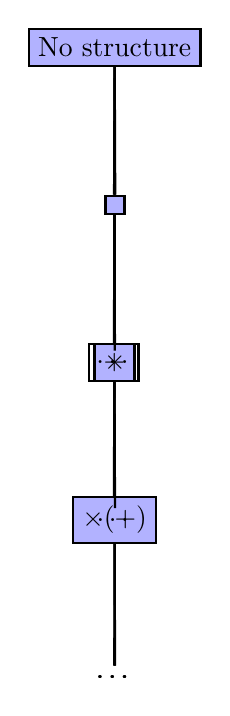
\begin{tikzpicture}
[sibling distance=0.15\treescale,-,thick, level distance=2cm]
%\footnotesize
\node[shape=rectangle,draw,thick,fill=blue!30] {No structure}
  child {node[shape=rectangle,draw,thick] {$\SE$}
  }
  child {node[shape=rectangle,draw,thick,fill=blue!30] {$\RQ$}
    [sibling distance=0.1\treescale]
    child {node[shape=rectangle,draw,thick] {$\SE$ + \RQ}}
    child {node {\ldots}}
    child {node[shape=rectangle,draw,thick,fill=blue!30] {$\Per + \RQ$}
      [sibling distance=0.15\treescale]
      child {node[shape=rectangle,draw,thick] {$\SE + \Per + \RQ$}}
      child {node {\ldots}}
      child {node[shape=rectangle,draw,thick,fill=blue!30] {$\SE \times (\Per + \RQ)$}
        [sibling distance=0.14\treescale]
        child {node {\ldots}}
        child {node {\ldots}}
        child {node {\ldots}}
      }
      child {node {\ldots}}
    }
    %child {node {$\RQ \times \SE$}}
    child {node {\ldots}}
    child {node[shape=rectangle,draw,thick] {$\Per \times \RQ$}}
  }
  child {node[shape=rectangle,draw,thick] {$\Lin$}
  }
  child {node[shape=rectangle,draw,thick] {$\Per$}
  };
\end{tikzpicture}
%\end{minipage} & 
%\newcommand{\wmgt}{3.4cm}  % width maunu growth tree
%\newcommand{\hmgt}{3.2cm}  % height maunu growth tree
%\begin{minipage}[t][14cm][t]{0.3\columnwidth}
%\raisebox{6cm}{
%\begin{tabular}{c}
%\hspace{-0.3cm} \includegraphics[width=\wmgt,height=\hmgt]{\grammarfiguresdir/decomposition/11-Feb-v4-03-mauna2003-s_max_level_0/03-mauna2003-s_all_small} \\
%\hspace{-0.3cm} \includegraphics[width=\wmgt,height=\hmgt]{\grammarfiguresdir/decomposition/11-Feb-v4-03-mauna2003-s_max_level_1/03-mauna2003-s_all_small} \\
%\hspace{-0.3cm} \includegraphics[width=\wmgt,height=\hmgt]{\grammarfiguresdir/decomposition/11-Feb-v4-03-mauna2003-s_max_level_2/03-mauna2003-s_all_small}
%\end{tabular}
%}
%\end{minipage}
%\end{tabular}
\caption[Search tree over kernels]{An example of a search tree over kernel expressions.  Figure \ref{fig:mauna_grow} shows the model increasing in sophistication as the kernel expression grows.}
\label{fig:mauna_search_tree}
\end{figure}





\section{Model Evaluation}

Choosing kernel structures requires a criterion for evaluating structures.
We choose marginal likelihood as our criterion, since it balances the fit and complexity of a model \citep{rasmussen2001occam}.
Conditioned on kernel parameters, the marginal likelihood of a \gp{} can be computed analytically.
However, to evaluate a kernel family we must integrate over kernel parameters.
We approximate this intractable integral with the Bayesian information criterion \citep{schwarz1978estimating} after first optimizing to find the maximum-likelihood kernel parameters.

In a fully Bayesian approach, we would put priors over the parameters and compute the marginal likelihood of the models with all the parameters integrated out.
However, as this would be difficult to do across our space of models, we approximate this integral by choosing the parameters to optimize the marginal likelihood, and then apply the Bayesian information criterion (BIC) to penalize model complexity.
%To avoid an expensive integration over kernel parameters, we used the Bayesian information criterion \citep{schwarz1978estimating} as an approximation.

Of course, other model selection criteria could be used with our search procedure.
For instance, cross-validation could be used when the goal is interpolation.


%\footnotetext{This is the heuristic used in chapter 5 of \citet{rasmussen38gaussian} when constructing a kernel to analyse the Mauna Loa dataset.}
% inspired by the same heuristic of extending models by examining residuals mentioned above.
%\begin{itemize}
%\item We (as researchers) often choose kernel structures by looking at the residuals and coming up with a model for those. This is analogous to applying rule (1), adding a new kernel but keeping the old parameters fixed.
%\item If a simple structure includes a periodic kernel, the learned period is likely to be approximately correct even if the true structure turns out to be more complex.
%\end{itemize}



We optimized kernel parameters at each step using conjugate gradients, randomly restarting any newly introduced kernel parameters.  To approximate the marginal likelihood of a kernel without integrating over parameters, used the Bayesian Information Criterion (\BIC{}) \citep{schwarz1978estimating}.
We also experimented with using the Laplace approximation to the marginal likelihood, but this was found to be less numerically stable and was not meaningful in cases when the optimiser failed to reach an optimum.
Because BIC is a function of the number of parameters in a model, we adjusted for cases where two parameters were only serving the role of one.  \eg when two kernels are multiplied, one of the variance parameters becomes redundant.

After each model is proposed its kernel parameters are optimised by conjugate gradient descent.
We evaluate each optimized model, $M$, using the Bayesian Information Criterion (\BIC{}) \citep{schwarz1978estimating}:
\begin{equation}
\textnormal{BIC}(M) = -2 \log p(D\given M) + p \log n
\end{equation}
where $p$ is the number of kernel parameters, $\log p(D|M)$ is the marginal likelihood of the data, $D$, and $n$ is the number of data points.
BIC trades off model fit against model complexity and implements what is known as ``Bayesian Occam's Razor'' \citep{rasmussen2001occam,mackay2003information}.





\section{Structure Discovery in Time Series}
\label{sec:time_series}

%In this section, we show on several time series datasets both the kernel expression found by our search, and the complete \gp{} posterior distribution implied by that kernel and the data.  
%We then also plot that same kernel and posterior decomposed into additive components.

To investigate our method's ability to discover structure, we ran the kernel search on several time-series.
%in order to test whether it learns plausible and interpretable structure. 
%For these datasets, we show both the best kernel expressions found in each stage of the search, and the complete posterior distribution implied by that kernel and the data. 
%Additionally, we show decompositions of the time series into superpositions of components as implied by the kernel structure.
%We pay special attention to the models' extrapolations beyond the range of observed data, since this is a strong test of the correctness of the learned structure.
%\NA{
%Our method discovers rich structure in these datasets, and produces plausible extrapolations.  
%}

%We further demonstrate that the discovered structures can be decomposed into sums of interpretrable components.  
%All kernels in our search space can equivalently be written as sums of products of base kernels by applying distributivity.
%For example,
As discussed in \Cref{ch:kernels}, a \gp{} whose kernel is a sum of kernels can be viewed as a sum of functions drawn from component \gp{}s.
This provides another method of visualizing the learned structures.
In particular, all kernels in our search space can be equivalently written as sums of products of base kernels by applying distributivity. For example,
%
\begin{align}
\SE \times (\RQ + \Lin) = \SE \times \RQ + \SE \times \Lin
\end{align}
%
We visualize the decompositions into sums of components using the formulae given in the appendix.
%By decomposing a kernel into a sum we are able to decompose .%, even when the learned kernel was not originally of this form.
%
%these decompositions can be interpreted as superpositions of causal processes.
%Details of computations are given in the appendix.
%
%\section{Decomposing a function}
%
%Sums of kernels were shown in section~\ref{sec:Structure} to correspond to sums of independent functions.
%By splitting kernel expressions found by our search algorithm into additive components, we can also decompose the \gp{} posterior over functions into a joint distribution over functions that are summed togther.
%This potentially allows us to probabilistically separate causally the independent processes that give rise to the data. 
%
%\TBD{RBG: It's not immediately obvious that this section is part of the experiments. Also, maybe consider moving it till after the quantitative comparisons?  It could be useful rhetorically to first ask, ``how well does our algorithm do,'' and then ``let's find out why it works.''}
%
The search was run to depth 10, using the base kernels from Section \ref{sec:Structure}.
%\NA{
%We consider this set of kernels since they are diverse, interpretable and through composition span a large space of priors on functions.
%}
%\footnotetext{\NA{Typically the highest scoring kernel was found at an earlier depth. We ran to a fixed depth to reduce the chance of the search stopping due to poor choices of random initial parameters for new kernels.}}


%\paragraph{Decomposing a superposition}

%In cases where the kernel expression contains any product of a sum, our software automatically expands out the expression into an equivalent sum of products.  This operation transforms the posterior into a more interpretable, but equivalent, form.

\label{sec:extrapolation}
\paragraph{Mauna Loa atmospheric CO$\mathbf{_{2}}$}


Using our method, we analyzed records of carbon dioxide levels recorded at the Mauna Loa observatory.
Since this dataset was analyzed in detail by \citet{rasmussen38gaussian}, we can compare the kernel chosen by our method to a kernel constructed by human experts.
%it serves as a test of our algorithm's ability to recover known structure.
%First, we revisit a dataset explored in \mbox{\cite{rasmussen38gaussian}}%, pages 120-126
%, where a kernel was hand-tailored to fit a \gp{} model to the dataset.




\begin{figure}
\newcommand{\wmgd}{0.5\columnwidth}  % width mauna decomp
\newcommand{\hmgd}{3.51cm}  % height mauna decomp
\newcommand{\mdrd}{\grammarfiguresdir/decomposition/11-Feb-03-mauna2003-s}  % mauna decomp results dir
\newcommand{\mbm}{\hspace{-0.2cm}}  % move back
\newcommand{\maunadgfx}[1]{\mbm \includegraphics[width=\wmgd,height=\hmgd, clip, trim=0mm 0mm 0mm 6mm]{\mdrd/03-mauna2003-s_#1}}
\begin{tabular}{cc}
\multicolumn{2}{c}{
\begin{tabular}{c}
Complete Model: 
$\kLin \times \kSE + \kSE \times ( \kPer + \RQ ) + \kWN$ \\
\maunadgfx{all}
\end{tabular}
} \\\\
%\multicolumn{2}{c}{Decomposition} \\
Long-term trend: $\Lin \times \SE$ & Yearly Periodic: $\SE \times \Per$ \\
\maunadgfx{1} & \maunadgfx{2_zoom} \\[1em]
Short-term deviation: $\SE \times \RQ$ & Noise: \kWN \\
\maunadgfx{3} & \maunadgfx{resid}
\end{tabular}
\caption[Model decomposition of the Mauna-Loa time-series]
{First row: The posterior on the Mauna Loa dataset, after a search of depth 10.  Subsequent rows show the automatic decomposition of the time series.  The decompositions shows long-term, yearly periodic, medium-term anomaly components, and residuals, respectively.  In the third row, the scale has been changed in order to clearly show the yearly periodic structure.}
\label{fig:mauna_decomp}
\end{figure}



Figure \ref{fig:mauna_grow} shows the posterior mean and variance on this dataset as the search depth increases.
While the data can be smoothly interpolated by a single base kernel model, the extrapolations improve dramatically as the increased search depth allows more structure to be included.

Figure \ref{fig:mauna_decomp} shows the 
%complete posterior of the 
final model chosen by our method, together with its decomposition into additive components.
The final model exhibits both plausible extrapolation and interpretable components: a long-term trend, annual periodicity and medium-term deviations; the same components chosen by \citet{rasmussen38gaussian}.
%The final model exhibits the same structure 
%The automatically chosen kernel contains the same components as \citet{rasmussen38gaussian}: a long-term trend, annual periodicity and medium-term deviations from the trend.
We also plot the residuals, showing that there is little obvious structure left in the data.  
%
%\NA{
%
%The decomposition is qualitatively identical to that constructed in \citet{rasmussen38gaussian}.
%On this example, our search procedure is able to automate this construction where previously two \gp{} experts devoted 4 pages of text and analysis to the development of a composite kernel.
%}


\begin{figure}[h]
\centering
\newcommand{\wmg}{0.31\columnwidth}  % width maunu growth
\newcommand{\hmg}{3.2cm}  % height maunu growth
\newcommand{\maunadecomp}[1]{\hspace{-0.3cm}
\includegraphics[width=\wmg,height=\hmg, clip,trim=0mm 0mm 0mm 7mm]{\grammarfiguresdir/decomposition/11-Feb-v4-03-mauna2003-s_max_level_#1/03-mauna2003-s_all_small}}
\begin{tabular}{ccc}
Level 1: & Level 2: & Level 3: \\
\RQ & $\SE \times (\Per + \RQ )$ & $ \SE + \SE \times (\Per + \RQ )$ \\[0.5em]
\maunadecomp{0} & \maunadecomp{2} & \maunadecomp{3} \\[0.5em]
\end{tabular}
\caption[Progression of models as the search depth increases]
{Posterior mean and variance for different depths of kernel search.  The dashed line marks the extent of the dataset.  In the first column, the function is only modeled as a locally smooth function, and the extrapolation is poor.  Next, a periodic component is added, and the extrapolation improves.  At depth 3, the kernel can capture most of the relevant structure, and is able to extrapolate reasonably. %\TBD{RBG: (1) I think we somehow need to visualize the lengthscales, to make it obvious that the SE kernels really mean different things. (2) Why isn't SE + PE the correct answer?}
}
\label{fig:mauna_grow}
\end{figure}


\paragraph{Airline passenger data}

\begin{figure}[H]
\centering
\newcommand{\wagd}{0.48\columnwidth}  % width airline decomp
\newcommand{\hagd}{4cm}  % height airline decomp
\newcommand{\mb}{\hspace{-0.2cm}}  % move back
%\newcommand{\ard}{../figures/decomposition/11-Feb-01-airline-s}  % airline results dir
%\newcommand{\ard}{\grammarfiguresdir/decomposition/31-Jan-v301-airline-months}  % airline results dir
\newcommand{\ard}{\grammarfiguresdir/decomposition/19-Jan-2014-airline-months}  % airline results dir
\newcommand{\airdgfx}[1]{\mb \includegraphics[width=\wagd,height=\hagd, clip, trim=10mm 0mm 14mm 8mm]{\ard/#1} }
%
\begin{tabular}{cc}
\multicolumn{2}{c}{
\begin{tabular}{c}
Complete Model \\
\airdgfx{01-airline_all}
\end{tabular}
} \\
%\multicolumn{2}{c}{Decomposition} \\
Long-term trend & Yearly Periodic \\
 \airdgfx{01-airline_1_extrap} & \airdgfx{01-airline_2_extrap}\\
 Short-term deviation & Noise \\
 \airdgfx{01-airline_3_extrap} & \airdgfx{01-airline_4_extrap}
\end{tabular}
\caption[Decomposition of model discovered on airline dataset]
{First row:  The airline dataset and posterior after a search of depth 10.  Subsequent rows: Additive decomposition of posterior into long-term smooth trend, yearly variation, and short-term deviations.  Due to the linear kernel, the marginal variance grows over time, making this a heteroskedastic model. 
}
\label{fig:airline_decomp}
\end{figure}

Figure \ref{fig:airline_decomp} shows the decomposition produced by applying our method to monthly totals of international airline passengers~\citep{box2011time}.
We observe similar components to the previous dataset: a long term trend, annual periodicity and medium-term deviations.
In addition, the composite kernel captures the near-linearity of the long-term trend, and the linearly growing amplitude of the annual oscillations.
%The discovery of linear structure allows for a growing uncertainty highly plausible extrapolation.\fTBD{Mention heteroskedasticity?}

%Discovering this linearity results in very plausible extrapolations of the data.
%Figure~\ref{fig:airline_grow} demonstrates this by ploting the full posterior of the kernel discovered at sequential levels of the search.
%The first plot shows that the first kernel has discovered onyl short term continuity.
%The second kernel discovers periodicity that varies with time.
%The third kernel has discovered that the periodicity is growing approximately linearly.
%Finally, the fourth kernel has split the data into an approximately linear trend and growing oscillations.

%\begin{figure}[h!]
%\centering
%\newcommand{\wag}{4.8cm}  % width airline growth
%\newcommand{\hag}{4cm}  % height airline growth
%\begin{tabular}{cc}
%\includegraphics[width=\wag,height=\hag]{../figures/decomposition/01-airline-s_max_level_0/01-airline-s_all_small}
%\hspace{-1cm} \includegraphics[width=\wag,height=\hag]{../figures/decomposition/01-airline-s_max_level_1/01-airline-s_all_small} \\
%\hspace{-1cm} \includegraphics[width=\wag,height=\hag]{../figures/decomposition/01-airline-s_max_level_2/01-airline-s_all_small} 
%\hspace{-1cm} \includegraphics[width=\wag,height=\hag]{../figures/decomposition/01-airline-s_max_level_3/01-airline-s_all_small}
%\end{tabular}
%\caption{Posterior mean and variance for different levels of kernel search on the airline dataset. \TBD{RBG: it looks like the figures on the left got clipped.}}
%\label{fig:airline_grow}
%\end{figure}

% Created by the command:
% postprocessing.make_all_1d_figures(folder='../results/31-Jan-1d/', prefix='31-Jan-v3', rescale=False)

%To evaluate the effectiveness of our method we performed two types of experiments.
%First, we examined the ability of our algorithm to discover useful structure in one-dimensional datasets.  Second, we examined the predictive performance of our model on multi-dimensional datasets.
% testing the ability of the algorithm to infer both an accurate regression function estimate and to produce an interpretable decomposition of a regression function.
%The accuracy experiments show that our method consistently matches or beats previous state of the art regression methods (\TBD{not yet statistically significantly within each experiment - more experiments currently running\ldots}).
%The decomposition experiments produce highly interpretable decompositions of time series data and highly plausible extrapolations; a particularly rare property of naively applied (linear) smoothers (\TBD{justify comment - e.g.~local linear is just linear, GP Sq-Exp nose dives towards the mean}).




%It is likely that our framework could be extended to capture nonstationary structure by adding a changepoint kernel \TBD{cite?}.

%\paragraph{Multidimensional decomposition}  Decomposition of multi-dimensional posteriors into sums of one-dimensional functions is possible as well, and was demonstrated in \cite{duvenaud2011additive11}.  \fTBD{Probably citing myself too much...}








\section{Related Work}
\label{sec:related-work}

\def\rwsheader{\subsubsection}
%\paragraph{Composite kernels in GP models} The technique of constructing composite kernels using sums and products of existing kernels was demonstrated in detail in Chapter 5 of \cite{rasmussen38gaussian}, where the resulting posterior mean was also decomposed into a sum of component-wise means, although the posterior variance was not.  While \cite{rasmussen38gaussian} manually explored several composite kernels for a particular dataset, our work automates this search process over a grammar of possible composite kernels.

%\paragraph{Gaussian process kernels}
%There has been significant work on constructing \gp{} kernels and analyzing their properties.
%This work is summarized in Chapter 4 of \cite{rasmussen38gaussian}. 

\rwsheader{Nonparametric regression in high dimensions}
Nonparametric regression methods such as splines, locally weighted regression, and \gp{} regression are popular because they are capable of learning arbitrary smooth functions of the data.
Unfortunately, they suffer from the curse of dimensionality: it is very difficult for the basic versions of these methods to generalize well in more than a few dimensions.
Applying nonparametric methods in high-dimensional spaces can require imposing additional structure on the model.

One such structure is additivity.
Generalized additive models (GAM) assume the regression function is a transformed sum of functions defined on the individual dimensions: $\expect[f(\vx)] = g\inv(\sum_{d=1}^D f_d(x_d))$.
%Generalized additive models \cite{hastie1990generalized} are models in which the function is modeled as a sum of functions defined on the individual dimensions: $\expect[f(\vx)] = \sum_{d=1}^D f_d(x_d)$.
These models have a limited compositional form, but one which is interpretable and often generalizes well.
In our grammar, we can capture analogous structure through sums of base kernels along different dimensions.

It is possible to add more flexibility to additive models by considering higher-order interactions between different dimensions. 
Additive Gaussian processes \cite{duvenaud2011additive11} are a \gp{} model whose kernel implicitly sums over all possible products of one-dimensional base kernels.  
\citet{plate1999accuracy} constructs a \gp{} with a composite kernel, summing an \kSE{} kernel along each dimension, with an SE-ARD kernel (\ie a product of \kSE{} over all dimensions).
Both of these models can be expressed in our grammar.

A closely related procedure is smoothing-splines ANOVA \cite{wahba1990spline, gu2002smoothing}.
This model is a linear combinations of splines along each dimension, all pairs of dimensions, and possibly higher-order combinations.
Because the number of terms to consider grows exponentially in the order, in practice, only terms of first and second order are usually considered.

Semiparametric regression \citep[e.g.][]{ruppert2003semiparametric} attempts to combine interpretability with flexibility by building  a composite model out of an interpretable, parametric part (such as linear regression) and a `catch-all' nonparametric part (such as a \gp{} with an SE kernel).
In our approach, this can be represented as a sum of \kSE{} and \kLin{}.

\rwsheader{Kernel learning}
There is a large body of work attempting to construct a rich kernel through a weighted sum of base kernels \citep[e.g.][]{christoudias2009bayesian, Bach_HKL}.
%, including \gp{} models. 
%\citet{Bach_HKL} uses a regularized optimization framework to learn a weighted sum over an exponential number of kernels.
While these approaches find the optimal solution in polynomial time, speed comes at a cost: the component kernels, as well as their hyperparameters, must be specified in advance.

Another approach to kernel learning is to learn an embedding of the data points. 
\citet{lawrence2005probabilistic} learns an embedding of the data into a low-dimensional space, and constructs a fixed kernel structure over that space.
%\NA{
This model is typically used in unsupervised tasks and requires an expensive integration or optimisation over potential embeddings when generalizing to test points.
%}
\citet{salakhutdinov2008using} use a deep neural network to learn an embedding;
%\NA{
this is a flexible approach to kernel learning but relies upon finding structure in the input density, p(\inputVar).
Instead we focus on domains where most of the interesting structure is in \function(\inputVar).
%}\fTBD{removed comment about interpretability}%; this is a flexible approach to kernel learning but potentially less interpretable.

\citet{diosan2007evolving} and \citet{bing2010gp} learn composite kernels for support vector machines and relevance vector machines, using genetic search algorithms.
%Our work goes beyond this prior work by demonstrating the structure implied by composite kernels, employing a Bayesian search criterion, and allowing for the automatic discovery of interpretable structure from data.
Our work employs a Bayesian search criterion, and goes beyond this prior work by demonstrating the interpretability of the structure implied by composite kernels, and how such structure allows for extrapolation.
%We build upon this work by demonstrating the structure implied by composite kernels, allowing for the automatic discovery of interpretable structure from data.
%We build upon this work by interpreting the structure of composite kernels, demonstrating the automatic discovery of interpretable structure from data.
%We build upon this work by 
%pointing out and demonstrating the interpretability of the structure implied by composite kernels, and demonstrating useful decompositions on several real datasets, as well as by examining extrapolation, structure recovery, and multidimensional regression.
%Our work extends theirs by examining the interpretable structure of the discovered kernels.


\rwsheader{Structure discovery}

There have been several attempts to uncover the structural form of a dataset by searching over a grammar of structures. For example, \cite{Schmidt2009b}, \cite{todorovski1997declarative} and \cite{washio1999discovering} attempt to learn parametric forms of equations to describe time series, or relations between quantities. Because we learn expressions describing the covariance structure rather than the functions themselves, we are able to capture structure which does not have a simple parametric form.

\citet{kemp2008discovery} learned the structural form of a graph used to model human similarity judgments.
Examples of graphs included planes, trees, and cylinders.
Some of their discrete graph structures have continous analogues in our own space; \eg $\SE_1 \times \SE_2$ and $\SE_1 \times \Per_2$ can be seen as mapping the data to a plane and a cylinder, respectively.

\citet{grosse2012exploiting} performed a greedy search over a compositional model class for unsupervised learning, using a grammar and a search procedure which parallel our own. This model class contained a large number of existing unsupervised models as special cases and was able to discover such structure automatically from data. Our work is tackling a similar problem, but in a supervised setting.


\rwsheader{Building Kernel Functions}
\cite{rasmussen38gaussian} devote 4 pages to manually constructing a composite kernel to model a time series of carbon dioxode concentrations.
In the supplementary material, we include a report automatically generated by \procedurename{} for this dataset; our procedure chose a model similar to the one they constructed by hand.
Other examples of papers whose main contribution is to manually construct and fit a composite \gp{} kernel are \cite{klenske2012nonparametric} and \cite{lloydgefcom2012}.

\citet{diosan2007evolving, bing2010gp} and \citet{kronberger2013evolution} search over a similar space of models as \procedurename{} using genetic algorithms but do not interpret the resulting models.
%Our procedure is based on the model construction method of \citet{DuvLloGroetal13} which automatically decomposed models but components were interpreted manually and the space of models searched over was smaller than that in this work.


\rwsheader{Kernel Learning}

Sparse spectrum \gp{}s \citep{lazaro2010sparse} approximate the spectral density of a stationary kernel function using delta functions which corresponds to kernels of the form $\sum \cos$.
Similarly, \citet{WilAda13} introduce spectral mixture kernels which approximate the spectral density using a scale-location mixture of Gaussian distributions corresponding to kernels of the form $\sum \kSE \times \cos$.
Both demonstrate, using Bochner's theorem \citep{bochner1959lectures}, that these kernels can approximate any stationary covariance function.
Our language of kernels includes both of these kernel classes (see table~\ref{table:motifs}).

There is a large body of work attempting to construct rich kernels through a weighted sum of base kernels called multiple kernel learning (MKL) \citep[e.g.][]{bach2004multiple}.
These approaches find the optimal solution in polynomial time but only if the component kernels and parameters are pre-specified.
We compare to a Bayesian variant of MKL in section~\ref{sec:numerical} which is expressed as a restriction of our language of kernels.

\rwsheader{Equation learning}
\cite{todorovski1997declarative}, \cite{washio1999discovering} and \cite{schmidt2009distilling} learn parametric forms of functions specifying time series, or relations between quantities.
In contrast, \procedurename{} learns a parametric form for the covariance, allowing it to model functions without a simple parametric form.



\rwsheader{nonparametric nonstationary covariance learning}

TODO: Add a lit review of nonparametric nonstationary covariance learning.

\rwsheader{Discovering interpretable structure}
Besides allowing faster learning and extrapolation, learning a more structured kernel sometimes has the added benefit of making the resulting model more intepretable.
This is a similar motivation as for the use of sparsity-inducing methods: on many real datasets, the signal can be well-predicted by some small subset of the inputs.
Identifying this subset allows both better generalization, and a more interpretable model.


\rwsheader{Searching over open-ended model spaces}

This work was inspired by previous successes at searching over open-ended model spaces: matrix decompositions \citep{grosse2012exploiting} and graph structures \citep{kemp2008discovery}.
In both cases, the model spaces were defined compositionally through a handful of components and operators, and models were selected using criteria which trade off model complexity and goodness of fit.
Our work differs in that our procedure automatically interprets the chosen model, making the results accessible to non-experts.

\rwsheader{Natural-language output}
To the best of our knowledge, our procedure is the first example of automatic description of nonparametric statistical models.
However, systems with natural language output have been built in the areas of video interpretation \citep{barbu2012video} and automated theorem proving \citep{GanesalingamG13}.



\subsection{Comparison to equation learning}
\label{sec:eqn-learning-comp}

We now compare the descriptions generated by \procedurename{} to parametric functions produced by an equation learning system.
We show equations produced by Eureqa \citep{Eureqa} for the data sets shown above, using the default mean absolute error performance metric.

The learned function for the solar irradiance data is
\begin{align*}
\textrm{Irradiance($t$)} = 1361 + \alpha\sin(\beta + \gamma t)\sin(\delta + \epsilon t^2 - \zeta t)
\end{align*}
where $t$ is time and constants are replaced with symbols for brevity.
This equation captures the constant offset of the data, and models the long-term trend with a product of sinusoids, but fails to capture the solar cycle or the Maunder minimum.

The learned function for the airline passenger data is
\begin{align*}
\textrm{Passengers($t$)} = \alpha t + \beta\cos(\gamma - \delta t)\textrm{logistic}(\epsilon t - \zeta) - \eta
\end{align*}
which captures the approximately linear trend, and the periodic component with approximately linearly (logistic) increasing amplitude.
However, the annual cycle is heavily approximated by a sinusoid and the model does not capture heteroscedasticity.





\section{Predictive Accuracy}
\label{sec:numerical}


\subsection{Interpretability versus accuracy}

BIC trades off model fit and complexity by penalizing the number of parameters in a kernel expression.
This can result in \procedurename{} favoring kernel expressions with nested products of sums, producing descriptions involving many additive components.
While these models have good predictive performance the large number of components can make them less interpretable.
We experimented with distributing all products over addition during the search, causing models with many additive components to be more heavily penalized by BIC.
We call this procedure \procedurename{}-interpretability, in contrast to the unrestricted version of the search, \procedurename{}-accuracy.



%In addition to our demonstration of the interpretability of \procedurename{}, we compared the predictive accuracy of various model-building algorithms at interpolating and extrapolating time-series.
%\procedurename{} outperforms the other methods on average.



\subsection{Data sets}

We evaluate the performance of the algorithms listed below on 13 real time-series from various domains from the time series data library \citep{TSDL}; plots of the data can be found at the beginning of the reports in the supplementary material.



\subsection{Algorithms}

We compare \procedurename{} to equation learning using Eureqa \citep{Eureqa} and six other regression algorithms: linear regression, \gp{} regression with a single $\kSE$ kernel (squared exponential), a Bayesian variant of multiple kernel learning (MKL) \citep[e.g.][]{bach2004multiple}, change point modeling \citep[e.g.][]{garnett2010sequential, saatcci2010gaussian, FoxDunson:NIPS2012}, spectral mixture kernels \citep{WilAda13} (spectral kernels) and trend-cyclical-irregular models \citep[e.g.][]{lind2006basic}.

We use the default mean absolute error criterion when using Eureqa.
All other algorithms can be expressed as restrictions of our modeling language (see table~\ref{table:motifs}) so we perform inference using the same search methodology and selection criterion\footnotemark~with appropriate restrictions to the language.
For MKL, trend-cyclical-irregular and spectral kernels, the greedy search procedure of \procedurename{} corresponds to a forward-selection algorithm.
For squared exponential and linear regression the procedure corresponds to marginal likelihood optimisation.
More advanced inference methods are typically used for changepoint modeling but we use the same inference method for all algorithms for comparability.
\footnotetext{We experimented with using unpenalised marginal likelihood as the search criterion but observed overfitting, as is to be expected.} 

We restricted to regression algorithms for comparability; this excludes models which regress on previous values of times series, such as autoregressive or moving-average models \citep[e.g.][]{box2013time}.
Constructing a language for this class of time-series model would be an interesting area for future research.



\subsection{Extrapolation}

To test extrapolation we trained all algorithms on the first 90\% of the data, predicted the remaining 10\% and then computed the root mean squared error (\RMSE{}).
The \RMSE{}s are then standardised by dividing by the smallest \RMSE{} for each data set so that the best performance on each data set will have a value of 1.

%\begin{minipage}{\textwidth}
%\begin{figure}
%\begin{minipage}{\textwidth}
%\makebox[\textwidth]{
\hspace{-6mm}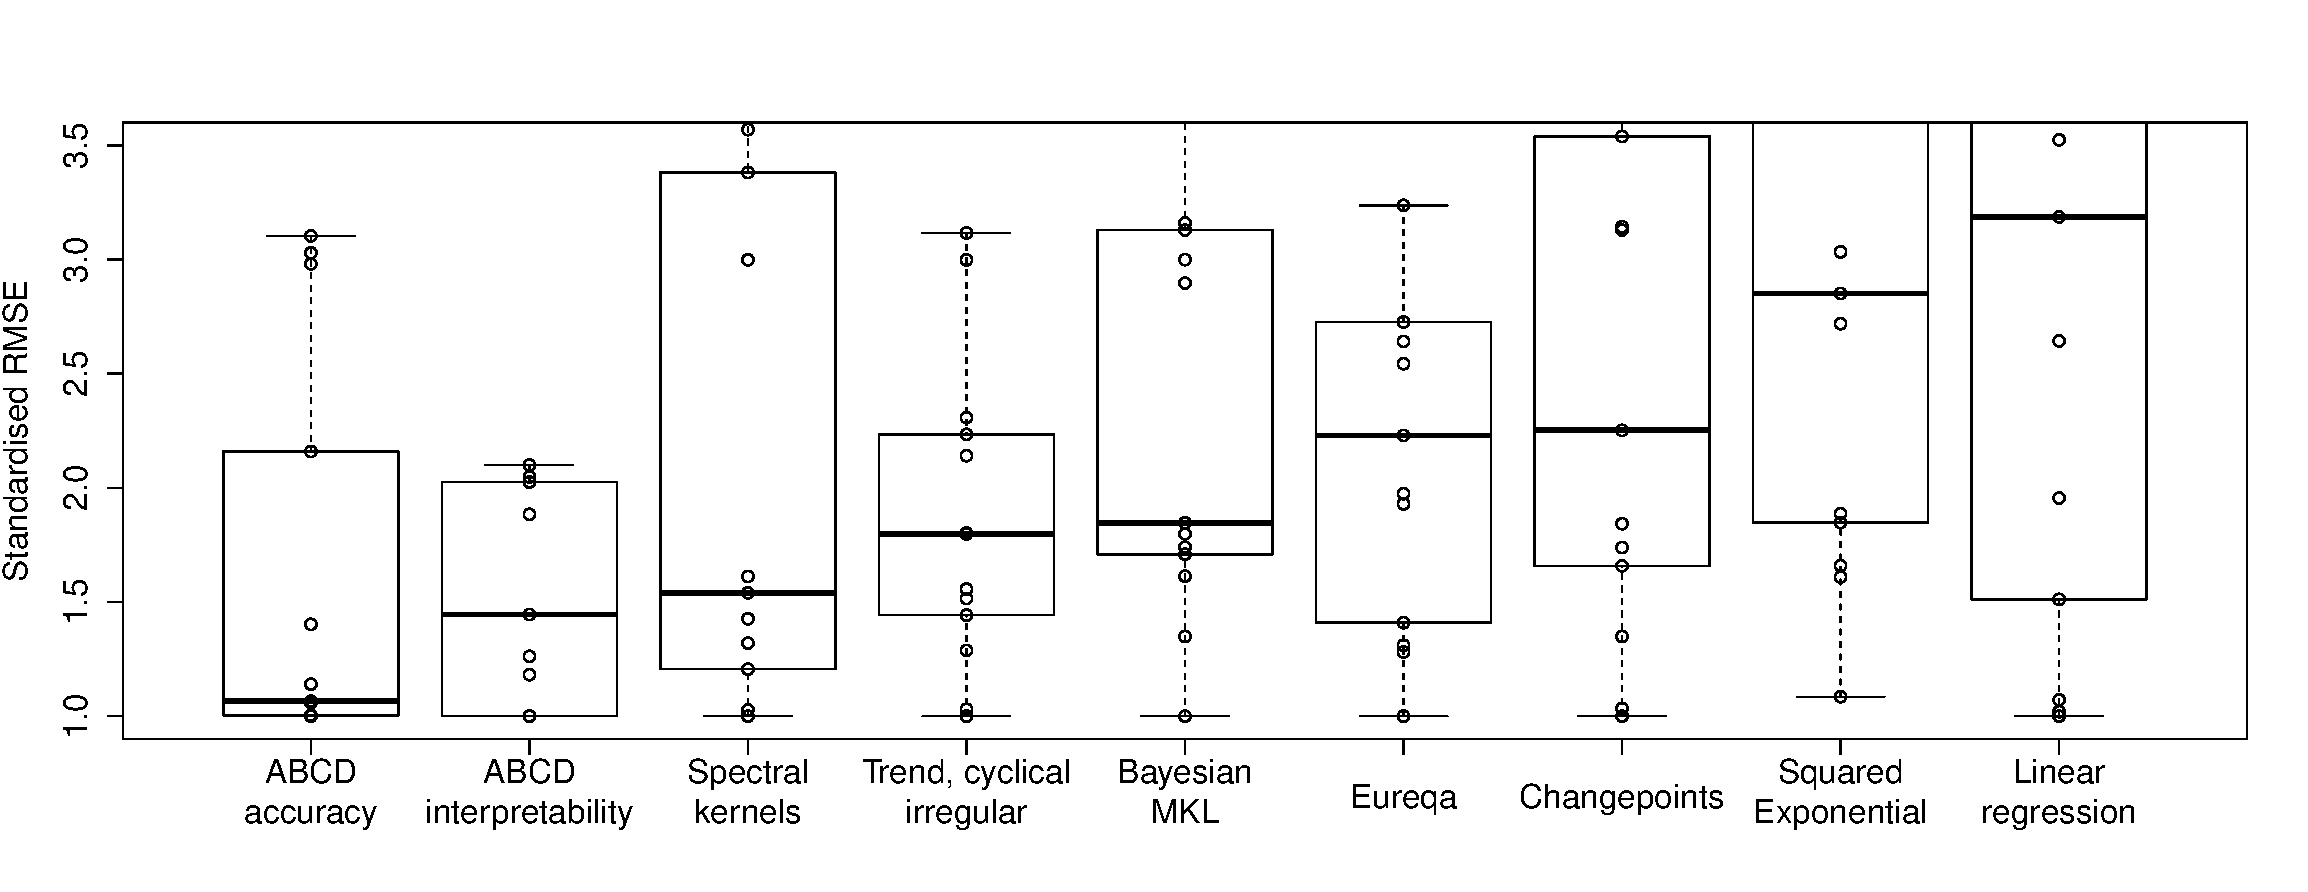
\includegraphics[width=1.02\textwidth]{\grammarfiguresdir/comparison/box_extrap_wide}
\captionof{figure}[Comparision of extrapolation error of all methods on 13 time-series datasets.]
{Box plot (showing median and quartiles) of standardised extrapolation RMSE (best performance = 1) on 13 time-series.
The methods are ordered by median.
}
\label{fig:box_extrap_dist}
%\end{figure}
%\end{minipage}

Figure~\ref{fig:box_extrap_dist} shows the standardised RMSEs across algorithms.
\procedurename{}-accuracy outperforms \procedurename{}-interpretability but both versions have lower quartiles than all other methods.

Overall, the model construction methods with greater capacity perform better: \procedurename{} outperforms trend-cyclical-irregular, which outperforms Bayesian \MKL{}, which outperforms squared exponential.
Despite searching over a rich model class, Eureqa performs relatively poorly, since very few datasets are parsimoniously explained by a parametric equation.

Not shown on the plot are large outliers for spectral kernels, Eureqa, squared exponential and linear regression with values of 11, 493, 22 and 29 respectively.
All of these outliers occurred on a data set with a large discontinuity (see the call centre data in the supplementary material).

\paragraph{Interpolation}
To test the ability of the methods to interpolate, we randomly divided each data set into equal amounts of training data and testing data.
The results are similar to those for extrapolation and are included in the appendix.




%\section{Quantitative evaluation}
%\label{sec:quantitative}

%In addition to producing highly interpretable decompositions of regression functions, our method also produces state of the art predictions in both extrapolation and interpolation tasks.
%In addition to the qualitative evaluation in section \ref{sec:time_series}, we investigated quantitatively how our method performs on both extrapolation and interpolation tasks.



%\fTBD{Josh: Can you write about the Blessing of abstraction, and doing lots with a small amount of data?  This might become apparent from plotting the extraplolations.}
%\fTBD{RBG: We could make this point as part of the learning curves for extrapolation by marking the points at which each additional aspect of the structure is found.}

\section{High-dimensional Prediction}

\procedurename{} can also be applied to multidimensional regression problems.
%
To evaluate the predictive accuracy of our method in a high-dimensional setting, we extended the comparison of \cite{duvenaud2011additive11} to include our method.
We performed 10-fold cross validation on 5 datasets,
\footnote{The data sets had dimensionalities ranging from 4 to 13, and the number of data points ranged from 150 to 450.} comparing 5 methods in terms of \MSE{} and predictive likelihood.
%\NA{
Our structure search was run up to depth 10, using the \SE{} and \RQ{} base kernel families.
%different subsets of the base kernel families.
%}

The comparison included three methods with fixed kernel families: Additive \gp{}s, Generalized Additive Models (\GAM{}), and a \gp{} with a standard \kSE{} kernel using Automatic Relevance Determination (\gp{} \kSE{}-\ARD{}).  Also included was the related kernel-search method of Hierarchical Kernel Learning (\HKL{}).
%We compared 5 methods on 5 datasets in terms of mean-squared (MSE) error and predictive likelihood, averaging across 10 data folds.

Results are presented in table \ref{tbl:Regression Mean Squared Error}.
%
% --- Automatically generated by resultsToLatex2.m ---
% Exported at 28-Jan-2013 15:53:45
\begin{table}[h]
\vspace{-0.1cm}
\caption[Comparison of multidimensional regression performance]
{Comparison of multidimensional regression performance.
Bold results are not significantly different from the best-performing method in each experiment, in a paired t-test with a $p$-value of 5\%.
}
\label{tbl:Regression Mean Squared Error}
{\small
\begin{center}
\begin{tabularx}{\textwidth}{l | XXXXX | XXXXX}
 & \multicolumn{5}{c}{Mean Squared Error (\MSE{})} & \multicolumn{5}{c}{Negative Log-Likelihood} \\
 Method & bach & \hspace{-3mm}\parbox{1cm}{concrete} & puma & servo & \hspace{-3mm}\parbox{1cm}{housing}
& bach  & \hspace{-3mm}\parbox{1cm}{concrete} & puma & servo & \hspace{-3mm}\parbox{1cm}{housing}
\\ \hline
Linear reg.
& $1.031$ & $0.404$ & $0.641$ & $0.523$ & $0.289$
& $3.430$ & $1.403$ & $1.881$ & $2.678$ & $1.052$ \\
\GAM
& $1.259$ & $0.149$ & $0.598$ & $0.281$ & $0.161$ 
& $2.708$ & $0.467$ & $1.195$ & $1.800$ & $0.457$ \\
\HKL
& $\mathbf{0.199}$ & $0.147$ & $0.346$ & $0.199$ & $0.151$ 
& - & - & - & - & -\\
\gp{} \acro{\kSE{}-\ARD{}}
& $\mathbf{0.045}$ & $0.157$ & $\mathbf{0.317}$ & $\mathbf{0.126}$ & $\mathbf{0.092}$
& $\mathbf{0.869}$ & $0.398$ & $\mathbf{0.843}$ & $1.429$ & $0.207$ \\
Additive \gp{}
& $\mathbf{0.045}$ & $\mathbf{0.089}$ & $\mathbf{0.316}$ & $\mathbf{0.110}$ & $0.102$
& $\mathbf{0.869}$ & $\mathbf{0.114}$ & $\mathbf{0.841}$ & $1.309$ & $0.194$ \\
\hline
%$\SE{}$ 
%Structure Search & & &&&&&&&&\\
%& $\mathbf{0.044}$ & $0.089$ & $\mathbf{0.315}$ & $\mathbf{0.101}$ & $\mathbf{0.092}$ 
%& $\mathbf{-0.141}$ & $\mathbf{0.054}$ & $\mathbf{0.840}$ & $0.249$ & $\mathbf{0.147}$ \\
%\multirow{2}{1cm}{Search - $\SE{}, \RQ{}$}
%\begin{tabular}{@{}l@{}}Search \\ $\SE{}, \RQ{}$\end{tabular}
$\SE{}, \RQ{}$ Search
& $\mathbf{0.044}$ & $\mathbf{0.087}$ & $\mathbf{0.315}$ & $\mathbf{0.102}$ & $\mathbf{0.082}$
& $\mathbf{0.859}$ & $\mathbf{0.065}$ & $\mathbf{0.840}$ & $1.265$ & $\mathbf{0.059}$ \\
% - All kernels%$\SE{}, \RQ{}, \Lin{}, \Per{}$
%\begin{tabular}{@{}l@{}}Structure Search \\ $\SE{}, \RQ{}, \Lin{}, \Per{}$\end{tabular}
$\SE{}, \RQ{}, \Lin{}, \Per{}$
& $\mathbf{0.509}$ & $\mathbf{0.079}$ & $\mathbf{0.321}$ & $\mathbf{0.094}$ & $\mathbf{0.112}$
& $\mathbf{1.357}$ & $\mathbf{0.114}$ & $\mathbf{0.837}$ & $\mathbf{0.573}$ & $\mathbf{0.151}$ \\
\end{tabularx}
\end{center}
}
\end{table}
% End automatically generated LaTeX
%
Our method with all base kernels was always the best performing method, or the difference in performance was not statiscally significant at the 5\% level.


%Results are presented in table \ref{tbl:Regression Mean Squared Error}.
%Although not statistically significant, increasing the number of base kernels did not always increase the performance of the search, suggesting scope for improvement.
%
%All bold results are not significantly different from the best-performing method in each experiment in a paired t-test with a $p$-value of 5\%.
%
%% --- Automatically generated by resultsToLatex2.m ---
% Exported at 28-Jan-2013 15:53:45
\begin{table*}[ht!]
\caption{{\small
Regression Mean Squared Error
}}
\label{tbl:Regression Mean Squared Error}
\begin{center}
\begin{tabular}{l | r r r r r}
Method & \rotatebox{0}{ bach  }  & \rotatebox{0}{ concrete  }  & \rotatebox{0}{ puma }  & \rotatebox{0}{ servo }  & \rotatebox{0}{ housing }  \\ \hline
Linear Regression & $1.031$ & $0.404$ & $0.641$ & $0.523$ & $0.289$ \\
GP GAM & $1.259$ & $0.149$ & $0.598$ & $0.281$ & $0.161$ \\
HKL & $\mathbf{0.199}$ & $0.147$ & $0.346$ & $0.199$ & $0.151$ \\
GP Squared-exp & $\mathbf{0.045}$ & $0.157$ & $0.317$ & $0.126$ & $\mathbf{0.092}$ \\
GP Additive & $\mathbf{0.045}$ & $\mathbf{0.089}$ & $\mathbf{0.316}$ & $\mathbf{0.110}$ & $0.102$ \\
%22-Jan & $\mathbf{0.513}$ & $\mathbf{0.089}$ & $\mathbf{0.312}$ & $\mathbf{0.095}$ & $\mathbf{0.091}$ \\
\hline
Structure Search & $\mathbf{0.044}$ & $\mathbf{0.087}$ & $\mathbf{0.315}$ & $\mathbf{0.102}$ & $\mathbf{0.082}$
\end{tabular}
\end{center}
\end{table*}
% End automatically generated LaTeX

%% --- Automatically generated by resultsToLatex2.m ---
% Exported at 28-Jan-2013 15:53:45
\begin{table*}[ht!]
\caption{{\small
Regression Negative Log Likelihood
}}
\label{tbl:Regression Negative Log Likelihood}
\begin{center}
\begin{tabular}{l | r r r r r}
Method & \rotatebox{0}{ bach  }  & \rotatebox{0}{ concrete  }  & \rotatebox{0}{ puma }  & \rotatebox{0}{ servo }  & \rotatebox{0}{ housing }  \\ \hline
Linear Regression & $2.430$ & $1.403$ & $1.881$ & $1.678$ & $1.052$ \\
GP GAM & $1.708$ & $0.467$ & $1.195$ & $0.800$ & $0.457$ \\
GP Squared-exp & $\mathbf{-0.131}$ & $0.398$ & $0.843$ & $0.429$ & $0.207$ \\
GP Additive & $\mathbf{-0.131}$ & $\mathbf{0.114}$ & $\mathbf{0.841}$ & $\mathbf{0.309}$ & $0.194$ \\
%22-Jan & $\mathbf{0.346}$ & $\mathbf{0.134}$ & $\mathbf{0.835}$ & $\mathbf{0.241}$ & $\mathbf{0.138}$ \\
\hline
Structure Search & $\mathbf{-0.141}$ & $\mathbf{0.065}$ & $\mathbf{0.840}$ & $\mathbf{0.265}$ & $\mathbf{0.059}$
\end{tabular}
\end{center}
\end{table*}
% End automatically generated LaTeX

%
%\fTBD{Is it worth including the learned structures in the table?}
%\paragraph{Details of methods}
%Linear regression was included as a baseline, with noise variance set to the empirical variance on the training residuals.
%
%Generalized Additive Models (GP GAM) were implemented through a \gp{} whose kernel is a sum of \kSE{} kernels across dimensions.
%This model was included to demonstrate that the gain in predictive performance was not simply due to the inclusion of additive structure.
%
%Additive \gp{} was run using \kSE{} as a base kernel, with at most ten degrees of interaction.
%
%Hierarchical Kernel Learning (HKL)
%\footnote{Code for HKL available at \texttt{http://www.di.ens.fr/\textasciitilde fbach/hkl/}} 
%was run using the all-subsets kernel, which corresponds to the same set of kernels as considered by the additive \gp{} with a \kSE{} base kernel.
%Because HKL does not produce a probabilistic prediction, it could not be included in Table \ref{tbl:Regression Negative Log Likelihood}.
%

%$k = 1$, $D = 8$, kernels are SE and RQ (\TBD{currently running other experiments that may be more canonical}).
%We have extended the comparison of \cite{duvenaud2011additive11} to include our method.

%Some points for discussion
%\begin{itemize}
%\item Experiments just using SE kernel can outperform additive kernel surprisingly. This is presumably a regularisation effect of using a finite depth search and/or BIC. We could make this a more Bayesian result (i.e.~more a property of the model) by placing a prior on kernels that depends on the number of components.
%\item Need to discuss design choices e.g.~$k$, depth of search, base kernels.
%\end{itemize}



\subsection{Validation on Synthetic Data}
\label{sec:synthetic}

Because it is difficult to visualize the structures discovered in multiple dimensions, it is difficult to tell from predictive accuracy alone if the search procedure is finding all structure present.
To address this questions, we validated our method's ability to recover known structure on a set of synthetic datasets.

For several composite kernel expressions, we constructed synthetic data by first sampling 300 points uniformly at random, then sampling function values at those points from a \gp{} prior.
%We then added \iid Gaussian noise to the function values, with variance chosen such that the standard deviation of the noise $\sigma_n$ relative to the sample variance of the function was 0.1.
We then added \iid Gaussian noise to the functions, at various signal-to-noise ratios (\SNR{}).

%\begin{table*}[ht!]
\caption{{\small
Kernels used to generate synthetic data together, dimensionality, $D$, of the input space and the inferred kernels at different signal to noise ratios (SNR).
The two kernels marked with an asterisk * indicate when the search procedure inferred extraneous structure.
}}
\label{tbl:synthetic}
\begin{center}
{\tiny
\begin{tabular}{c c | c c c c c}
Kernel & $D$ & SNR = 100 & SNR = 10 & SNR = 1 & SNR = 0.1 & SNR = 0.01 \\
\hline
$\SE + \RQ$                               & 1 & $\RQ$
                                              & $\SE$
                                              & $\SE \times \Per$*
                                              & $\SE$
                                              & - \\
$\Lin \times \Per$                        & 1 & $\Lin \times \Per$ 
                                              & $\Lin \times \Per$
                                              & $\Lin \times \Per$
                                              & $\SE$
                                              & - \\
$\SE_1 + \RQ_2$                           & 2 & $\SE_1 + \RQ_2$
                                              & $\SE_1 + \SE_2$
                                              & $\Lin_1 + \SE_2$ 
                                              & $\Lin_1$
                                              & - \\
$\SE_1 + \SE_2 \times \Per_1 + \SE_3$     & 3 & $\SE_1 + \SE_2 \times \Per_1 + \SE_3$
                                              & $\SE_1 + \SE_2 \times \Per_1 + \SE_3$
                                              & $\SE_2 \times \Per_1 + \SE_3$
                                              & -
                                              & - \\
$\SE_1 \times \SE_2$                      & 4 & $\SE_1 \times \SE_2 \times \Lin_1$
                                              & $\SE_1 \times \SE_2$
                                              & $\Lin_1 \times \SE_2$
                                              & $\Lin_2$
                                              & - \\
$\SE_1 \times \SE_2 + \SE_2 \times \SE_3$ & 4 & $\SE_1 \times \SE_2 + \SE_2 \times \SE_3$
                                              & $\SE_1 \times \SE_2 + \SE_2 \times \SE_3$
                                              & $\SE_1 + \SE_2 \times \SE_3$
                                              & $\SE_1$
                                              & - \\
$(\SE_1 + \SE_2) \times (\SE_3 + \SE_4)$  & 4 & $(\SE_1 + \SE_2) \times (\SE_3 + \SE_4\times\Lin_4)$
                                              & $(\SE_1 + \SE_2) \times (\SE_3\times\Lin_3\times\Lin_1 + \SE_4)$*
                                              & $(\SE_1 + \SE_2) \times \SE_3 \times \SE_4$
                                              & -
                                              & - \\
\end{tabular}
}
\end{center}
\end{table*}

%\begin{table*}[ht!]
\caption{{\small
%Kernels used to generate synthetic data, dimensionality, $D$, of the input space, and the estimated kernels.% at different signal to noise ratios (SNR).
Kernels chosen by our method on synthetic data generated using known kernel structures. $D$ denotes the dimension of the functions being modeled.  SNR indicates the signal-to-noise ratio. Dashes - indicate no structure.
%The two kernels marked with an asterisk * indicate when the search procedure inferred extraneous structure.
}}
\label{tbl:synthetic}
\begin{center}
{\small
\begin{tabular}{c c | c c c}
True Kernel & $D$ & SNR = 10 & SNR = 1 & \hspace{-1cm} SNR = 0.1 \\
\hline
$\SE + \RQ$                               & 1 
                                              & $\SE$
                                              & $\SE \times \Per$
                                              & $\SE$
                                              \\
$\Lin \times \Per$                        & 1 
                                              & $\Lin \times \Per$
                                              & $\Lin \times \Per$
                                              & $\SE$
                                              \\
$\SE_1 + \RQ_2$                           & 2 
                                              & $\SE_1 + \SE_2$
                                              & $\Lin_1 + \SE_2$ 
                                              & $\Lin_1$
                                              \\
$\SE_1 + \SE_2 \times \Per_1 + \SE_3$     & 3 
                                              & $\SE_1 + \SE_2 \times \Per_1 + \SE_3$
                                              & $\SE_2 \times \Per_1 + \SE_3$
                                              & -
                                              \\
$\SE_1 \times \SE_2$                      & 4 
                                              & $\SE_1 \times \SE_2$
                                              & $\Lin_1 \times \SE_2$
                                              & $\Lin_2$
                                              \\
$\SE_1 \times \SE_2 + \SE_2 \times \SE_3$ & 4 
                                              & $\SE_1 \times \SE_2 + \SE_2 \times \SE_3$
                                              & $\SE_1 + \SE_2 \times \SE_3$
                                              & $\SE_1$
                                              \\
$(\SE_1 + \SE_2) \times (\SE_3 + \SE_4)$  & 4 
                                              & $(\SE_1 + \SE_2) \times (\SE_3\times\Lin_3\times\Lin_1 + \SE_4)$
                                              & $(\SE_1 + \SE_2) \times \SE_3 \times \SE_4$
                                              & -
                                              \\
\end{tabular}
}
\end{center}
\end{table*}

\begin{table}[ht!]
\caption[Kernels chosen on synthetic data generated using known kernel structures]
{%Kernels used to generate synthetic data, dimensionality, $D$, of the input space, and the estimated kernels.% at different signal to noise ratios (SNR).
Kernels chosen by our method on synthetic data generated using known kernel structures. $D$ denotes the dimension of the functions being modeled.  SNR indicates the signal-to-noise ratio. Dashes - indicate no structure was found.
%The two kernels marked with an asterisk * indicate when the search procedure inferred extraneous structure.
}
\label{tbl:synthetic}
\begin{center}
{\small
\begin{tabular}{c c | c c c}
True Kernel & $D$ & \SNR{} = 10 & \SNR{} = 1 & \hspace{-1cm} \SNR{} = 0.1 \\
\hline
$\SE + \RQ$        & 1 & $\SE$ & $\SE \times \Per$ & $\SE$ \\
$\Lin \times \Per$ & 1 & $\Lin \times \Per$ & $\Lin \times \Per$ & $\SE$ \\
$\SE_1 + \RQ_2$    & 2 & $\SE_1 + \SE_2$ & $\Lin_1 + \SE_2$ & $\Lin_1$ \\
$\SE_1 + \SE_2 \times \Per_1 + \SE_3$ & 3 & $\SE_1 + \SE_2 \times \Per_1 + \SE_3$ & $\SE_2 \times \Per_1 + \SE_3$ & - \\
$\SE_1 \times \SE_2$ & 4 & $\SE_1 \times \SE_2$ & $\Lin_1 \times \SE_2$ & $\Lin_2$ \\
$\SE_1 \times \SE_2 + \SE_2 \times \SE_3$ & 4 & $\SE_1 \times \SE_2 + \SE_2 \times \SE_3$ & $\SE_1 + \SE_2 \times \SE_3$ & $\SE_1$ \\
\multirow{2}{*}{ $(\SE_1 + \SE_2) \times (\SE_3 + \SE_4)$ } & \multirow{2}{*}{4} & $(\SE_1 + \SE_2) \times$ \dots & $(\SE_1 + \SE_2) \times$ \dots & \multirow{2}{*}{-} \\
 & & $(\SE_3\times\Lin_3\times\Lin_1 + \SE_4)$ & $\SE_3 \times \SE_4$ &
\end{tabular}
}
\end{center}
\end{table}

%\footnotetext{We define the signal to noise ratio to be the sample variance of the function divided by the variance of the noise.}
%
%
%Table~\ref{tbl:synthetic-less} lists the composite kernels we used to generate data (subscripts indicate which dimension each kernel was applied to), the dimensionality $D$ of the input space, the kernel chosen by our search, and the estimated noise variance.

%Our method finds all of the relevant structure in all but one test.
%In fact, it also discovers unintentionally introduced linear structure: functions sampled from \kSE{} kernels with long length scales occasionally resulted in near-linear trends in the data.

%The estimated noise level $\sigma_n$ numerically assesses the quality of the fit to the data; large positive or negative deviations from 0.1 would indicate under-fitting and over-fitting, respectively.
%The values reported show that the model is not severely over- or under-fitting.

%\paragraph{Not for paper - annoying results - to be included if a fix is found}

%Table~\ref{tbl:synthetic} shows the same experiment with different signal to noise ratios.
%We were hoping to see simpler kernels.
%The kernels \emph{are} simpler, but \kPer{} kernels have been sprinkled in.
%The parameters of these spurious kernels are extreme and they do not affect the kernel structure greatly - but they distract the reader.
%Future work could have elegant fixes for these problems (we are generating plenty of ideas as we go but the deadline is looking), for the time being we will try some heuristics (\eg do not display if it contributes a small (in some sense) amount to the total variation of the kernel).

Table~\ref{tbl:synthetic} shows the results.
The first column lists the true kernels we used to generate the data.
Subscripts indicate which dimension each kernel was applied to.
Subsequent columns show the dimensionality $D$ of the input space, and the kernels chosen by our search for different \SNR{}s.
Dashes - indicate that no kernel had a higher marginal likelihood than modeling the data as \iid Gaussian noise. % (\ie equivalent to a constant kernel).

%\NA{
For the highest \SNR{}, the method finds all relevant structure in all but one case.
The reported additional linear structure is explainable by the fact that functions sampled from \kSE{} kernels with long length scales occasionally have near-linear trends.
%}
%
%\NA{
%As the SNR lowers, the kernel expressions generally become simpler.
As the noise increases, our method generally backs off to simpler structures, rather than over-fitting.
%Two kernels have been marked with an asterisk indicating that the search has inferred more complex and erroneous structure.
%For the first data set with $\textrm{SNR} = 1$, the search erroneously infers periodic structure.
%On examining the data set, and the posterior fit of this kernel, the data could certainly be argued to have ambiguous structure.
%}





\section{Discussion}

Towards the goal of automating statistical modeling we have presented a system which constructs an appropriate model from an open-ended language and automatically generates detailed reports that describe patterns in the data captured by the model.
We have demonstrated that our procedure can discover and describe a variety of patterns on several time series.
Our procedure's extrapolation and interpolation performance on time-series are state-of-the-art compared to existing model construction techniques.
We believe this procedure has the potential to make powerful statistical model-building techniques accessible to non-experts.

%There has developed a large and mature literature on automatic structure discovery in unsupervised settings \fTBD{citations including Josh}.  
%For example, searches over large model classes have been succesfully used in machine vision \cite{pinto2009high}, analogous to high-throughput methods used in biology.
%However, relatively little attention has been paid to automatic structure discovery in supervised learning.
%
%Our work respresents a step towards automated structure discover in supervised settings.
% data-based modeling, as opposed to proposing the model beforehand.

%In particular, this work removes the need for an expert to propose a kernel family in order to effectively use a Gaussian process model.  
%Choosing a kernel family is a stumbling block even for experts.
%Automating the search over kernel structures will make it easier for non-statisticians to construct appropriate models for their data.

%The ability to learn kernel parameters and combination weights automatically has been an important factor in enabling the widespread use of kernel methods.
%For the most part, however, it has been up to the user to choose the proper form for the kernel, a task which requires considerable expertise.

Towards the goal of automating the choice of kernel family, we introduced a space of composite kernels defined compositionally as sums and products of a small number of base kernels.  
The set of models included in this space includes many standard regression models.
We proposed a search procedure for this space of kernels which parallels the process of scientific discovery.

We found that the learned structures are often capable of accurate extrapolation in complex time-series datasets, and are competitive with widely used kernel classes and kernel combination methods on a variety of prediction tasks.
The learned kernels often yield decompositions of a signal into diverse and interpretable components, enabling model-checking by humans.  %provides an additional degree of reassurance that the learned structure reflects the world.
We believe that a data-driven approach to choosing kernel structures automatically can help make nonparametric regression and classification methods accessible to non-experts.



We hope that the \procedurename{} algorithm will help replace the current and often opaque art of kernel engineering with a more transparent science of automated kernel construction.

\section{Future work}

While we focus on Gaussian process regression, we believe our kernel search method can be extended to other supervised learning frameworks such as classification or ordinal regression, or to other kinds of kernel architectures such as kernel SVMs.


%\paragraph{Source Code}
%Source code to perform all experiments is available on github\footnotemark.
\footnote{
%\url{http://www.github.com/jamesrobertlloyd/gpss-research}. 
All \gp{} parameter optimisation was performed by automated calls to the GPML toolbox available at \url{http://www.gaussianprocess.org/gpml/code/}.}



\outbpdocument{
\bibliographystyle{plainnat}
\bibliography{references.bib}
}





\iffalse


\paragraph{Solar irradiance Data} 
Finally, we analyzed annual solar irradiation data from 1610 to 2011 \citep{lean1995reconstruction}.
%
\begin{figure}
\newcommand{\wsd}{0.5\columnwidth}  % width solar decomp
\newcommand{\hsd}{4cm}  % height solar decomp
\newcommand{\srd}{\grammarfiguresdir/decomposition/11-Feb-02-solar-s}  % solar decomp results dir
\newcommand{\mbs}{\hspace{-0.3cm}}  % move back
\begin{tabular}{cc}
\mbs 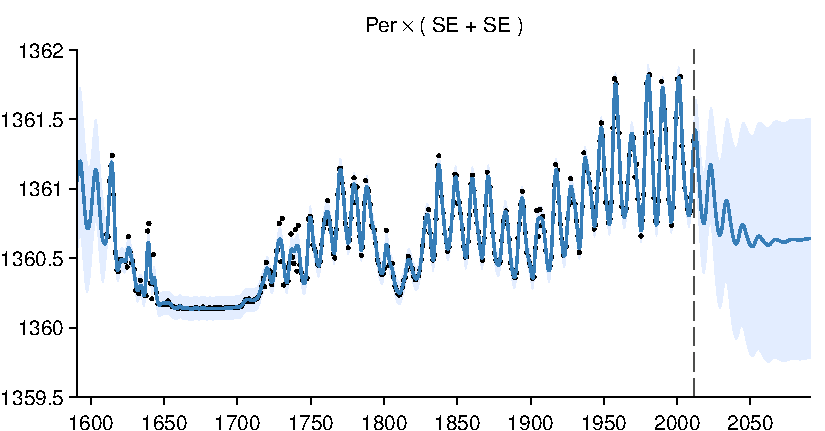
\includegraphics[width=\wsd,height=\hsd]{\srd/02-solar-s_all} &
\mbs 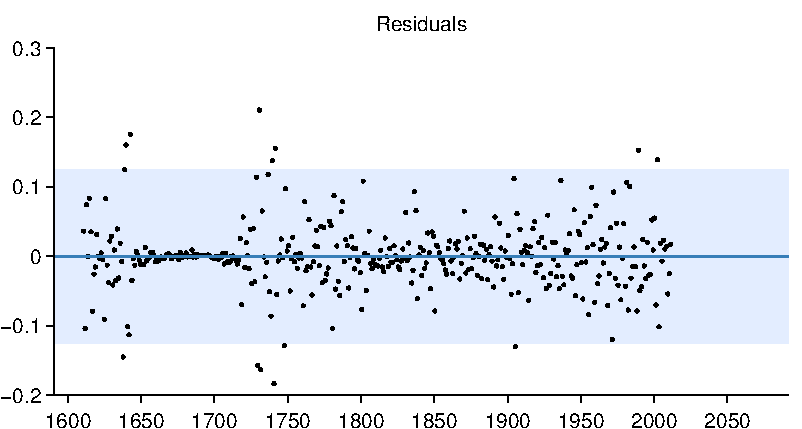
\includegraphics[width=\wsd,height=\hsd]{\srd/02-solar-s_resid}
\end{tabular}
\caption[Decomposition of model discovered on solar irradiance dataset]
{Full posterior and residuals on the solar irradiance dataset.}
\label{fig:solar_decomp}
\end{figure}
%
The posterior and residuals of the learned kernel are shown in figure \ref{fig:solar_decomp}.
%The composite kernel captures the periodic structure in the data, but does not capture the flat structure from 1645 to 1715 during which sunspots were extremely rare.
%but it misses out on another aspect of the data: the flat period from 1645 to 1715 which contains no periodicity and has much smaller variance than the rest of the dataset.
%This corresponds to the Maunder minimum, a period in which sunspots were extremely rare.
%
None of the models in our search space are capable of parsimoniously representing the lack of variation from 1645 to 1715. %, since all of the base kernels apart from \kLin{} are stationary.
%, and it is hard to see how Lin would help in modeling this structure.
%
%
Despite this, our approach fails gracefully: the learned kernel still captures the periodic structure, and the quickly growing posterior variance demonstrates that the model is uncertain about long term structure.
\fi


\iffalse

\subsection{Extrapolation}

\begin{figure}
\centering
\begin{tabular}{c}
\hspace{-0.5cm}
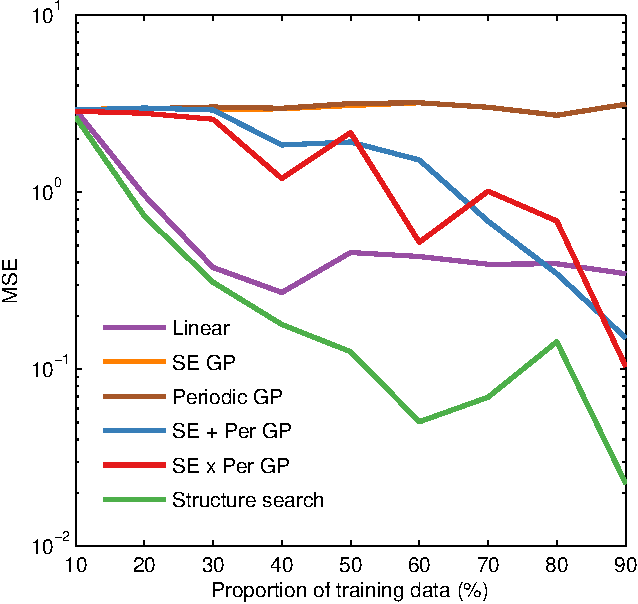
\includegraphics[width=0.5\columnwidth,height=7cm]{\grammarfiguresdir/extrapolation_curves/01-airline-s-ex-curve_hint.pdf}
\end{tabular}
\caption[Comparison of extrapolation performance]
{Extrapolation performance on the airline dataset.  We plot test-set MSE as a function of the fraction of the dataset used for training. 
%\TBD{RBG: Are we using a fixed test set, or the complement of the training set?  It seems like we should do the former, so that the results are less noisy.}
}
\label{fig:extrapolation}
\end{figure}

We compared the extrapolation capabilities of our model against standard baselines\footnotemark.
Dividing the airline dataset into contiguous training and test sets, we computed the predictive mean-squared-error (MSE) of each method.
We varied the size of the training set from the first 10\% to the first 90\% of the data.

Figure \ref{fig:extrapolation} shows the learning curves of linear regression, a variety of fixed kernel family \gp{} models, and our method.  
\gp{} models with only \kSE{} and \kPer{} kernels did not capture the long-term trends, since the best parameter values in terms of \gp{} marginal likelihood only capture short term structure. 
Linear regression approximately captured the long-term trend, but quickly plateaued in predictive performance.
The more richly structured \gp{} models (${\kSE + \kPer}$ and ${\kSE \times \kPer}$) eventually captured more structure and performed better, but the full structures discovered by our search outperformed the other approaches in terms of predictive performance for all data amounts.
%In contrast, a \gp{} with an SE or RQ kernel has unbounded capacity.  However, simply having unbounded capacity does not necessarily translate into the ability to extrapolate, as demonstrate in Figure \ref{fig:extrapolation}.  Only by increasing the amount of structure expressible in a model can we capture the regularities in the data that allow long-range extrapolation.

\footnotetext{
%\NA{
In one dimension, the predictive means of all baseline methods in table \ref{tbl:Regression Mean Squared Error} are identical to that of a \gp{} with an $\kSE{}$ kernel.}
%}

\fi


